%%%%%%%%%%%%%%%%%%%%%%%%%%%%%%%%%%%%%%%%%%%%%%%%%%%
%
%  New template code for TAMU Theses and Dissertations starting Spring 2021.
%
%
%  Last Updated: 1/13/2021
%
%%%%%%%%%%%%%%%%%%%%%%%%%%%%%%%%%%%%%%%%%%%%%%%%%%%

% THIS TEMPLATE IS THE MOST
% CURRENT. SEE THE FILES README.TXT AND NEWCHANGES.TXT
% FOR MORE INFORMATION.

\documentclass[12pt]{report}

\usepackage{tamuconfig}
\usepackage{array}
\usepackage{tabularx,booktabs}
\usepackage{listings}
\usepackage{xcolor}
\usepackage{subfig}
\definecolor{codegreen}{rgb}{0,0.6,0}
\definecolor{codegray}{rgb}{0.5,0.5,0.5}
\definecolor{codepurple}{rgb}{0.58,0,0.82}
\definecolor{backcolour}{rgb}{0.95,0.95,0.92}
\definecolor{lightgray}{rgb}{.9,.9,.9}
\definecolor{darkgray}{rgb}{.4,.4,.4}
\definecolor{purple}{rgb}{0.65, 0.12, 0.82}

%  for checkmark
\usepackage{amssymb}
\usepackage{multirow}


\setlength{\tabcolsep}{20pt}
\renewcommand{\arraystretch}{1.5}

\lstdefinestyle{Python}{
    backgroundcolor=\color{backcolour},
    commentstyle=\color{codegreen},
    keywordstyle=\color{magenta},
    numberstyle=\tiny\color{codegray},
    stringstyle=\color{codepurple},
    basicstyle=\ttfamily\footnotesize,
    breakatwhitespace=false,
    breaklines=true,
    captionpos=b,
    keepspaces=true,
    numbers=left,
    numbersep=5pt,
    showspaces=false,
    showstringspaces=false,
    showtabs=false,
    tabsize=2
}
\lstset{style=Python}


\lstdefinelanguage{JavaScript}{
  keywords={typeof, new, true, false, catch, function, return, null, catch, switch, var, if, in, while, do, else, case, break},
  keywordstyle=\color{blue}\bfseries,
  ndkeywords={class, export, boolean, throw, implements, import, this},
  ndkeywordstyle=\color{darkgray}\bfseries,
  identifierstyle=\color{black},
  sensitive=false,
  comment=[l]{//},
  morecomment=[s]{/*}{*/},
  commentstyle=\color{purple}\ttfamily,
  stringstyle=\color{red}\ttfamily,
  morestring=[b]',
  morestring=[b]"
}

\lstset{
   language=JavaScript,
   backgroundcolor=\color{lightgray},
   extendedchars=true,
   basicstyle=\tiny,
   showstringspaces=false,
   showspaces=false,
   numbers=left,
   numberstyle=\footnotesize,
   numbersep=5pt,
   tabsize=2,
   breaklines=true,
   showtabs=false,
   captionpos=b
}

\newcolumntype{L}{>{\centering\arraybackslash}m{3cm}}

% Most of the packages that set the default settings
% for the document have moved to the style file
% tamuconfig.sty. This includes

%These next lines change the font. Fixes for certain
%fonts will be implemented in a future release.

%Comment this line if you do not wish to use Times
%New Roman. The font used will then be the LaTeX
%default of Computer Modern.
\usepackage{times}
%\usepackage{cmbright}
\usepackage[T1]{fontenc}

% For natbib-style references, uncomment this.
%\usepackage{natbib}

%This package allows for the use of graphics in the
%document.
\usepackage{graphicx}

%If you have JPEG format images, add .jpg as an
%allowed file extension below. Same for Bitmaps (.bmp).
\DeclareGraphicsExtensions{.png}

%It is best practice to keep all your pictures in
%one folder inside the main directory in which your
%TeX file is kept. Here the folder is named "graphic."
%Replace the name here with your folder's name, if needed.
%The period is needed due to relative referencing.
\graphicspath{ {./figures/} }

% subfigure
\usepackage{subfig}

% For quick document navigation.
\usepackage[hidelinks]{hyperref}
\usepackage{nameref}
\newcounter{mylabelcounter}

\makeatletter
\newcommand{\labelText}[2]{%
#1\refstepcounter{mylabelcounter}%
\immediate\write\@auxout{%
  \string\newlabel{#2}{{1}{\thepage}{{\unexpanded{#1}}}{mylabelcounter.\number\value{mylabelcounter}}{}}%
}%
}
\makeatother


%%%%%%%%%%%%%%%%%%%%%%%%%%%%%%%%%%%%%%%%%%%%%%%%%%%%%%%%%
%Please place all your personal packages here. Check to
%see if the packages you wish to use are not already
%declared above. Placing all your personal packages
%here allows me to determine if there are any package
%issues in compilation, as well as any conflicts
%that may arise by the order of loading.
%
%%%%%%%%%%%%%%%%%%%%%%%%%%%%%%%%%%%%%%%%%%%%%%%%%%%%%%%%%
%%%%%%%%%%%%%%%%%%%%%%%%%%%%%%%%%%%%%%%%%%%%%%%%%%%%%%%%%
%Begin student defined packages.
%%%%%%%%%%%%%%%%%%%%%%%%%%%%%%%%%%%%%%%%%%%%%%%%%%%%%%%%%
%%%%%%%%%%%%%%%%%%%%%%%%%%%%%%%%%%%%%%%%%%%%%%%%%%%%%%%%%
%End student defined packages.
%%%%%%%%%%%%%%%%%%%%%%%%%%%%%%%%%%%%%%%%%%%%%%%%%%%%%%%%%

% End preamble. Document begins below.

\begin{document}
\providecommand{\tabularnewline}{\\}
\pagenumbering{roman} % Arabic numerals

\begin{titlepage}
    \begin{center}\large
        Gaming for Phishing Training: Teaching users to be safe through an interactive roleplaying game
        \vspace{5em}

        A Thesis

        \vspace{5em}

        \begin{singlespace}

            Submitted to the Graduate Faculty of the  \\
            University of New Orleans \\
            in partial fulfillment of the \\
            requirements for the degree of
        \end{singlespace}

        \vspace{5em}
        \begin{singlespace}
            Master of Science \\
            in \\
            Computer Science
        \end{singlespace}

        \vspace{5em}
        \par\end{center}
    \begin{center}\large
        \hspace{12pt} by \\
        \hspace{12pt} Saroj Duwal \\
        \hspace{12pt} B.S. University of New Orleans, 2019 \\
        \hspace{12pt} May, 2022\\


        \par\end{center}
\end{titlepage}
\pagebreak{}
\clearpage
\setcounter{page}{2}


 % This is simply a file that formats and adds your titlepage, please do not edit this unless you have a specific need. .

% \include{data/acknowledgements}

%%%%%%%%%%%%%%%%%%%%%%%%%%%%%%%%%%%%%%%%%%%%%%%%%%%%%%%%%%%%%%%%%%%%%%
%%       TABLE OF CONTENTS
%%%%%%%%%%%%%%%%%%%%%%%%%%%%%%%%%%%%%%%%%%%%%%%%%%%%%%%%%%%%%%%%%%%%%
% single-space sections in Table of Contents  - commented in version 1.7
%\renewcommand{\cftsecafterpnum}{\vskip0.5\baselineskip}
%\renewcommand{\cftsubsecafterpnum}{\vskip0.5\baselineskip}
%\renewcommand{\cftsubsubsecafterpnum}{\vskip0.5\baselineskip}
%%%%%%%%%%%%%%%%%%%%%%%%%%%%%%%%%%%%%%%%%%%%%%%%%%%

\phantomsection
% \addcontentsline{toc}{chapter}{Table of Contents}  
\renewcommand{\cftlottitlefont}{\center\Large}

\begin{singlespace}
\renewcommand\contentsname{\normalfont} {\centerline{\Large\bf{Table of Contents}}}

\setcounter{tocdepth}{4} % This puts \subsubsection[]{×} in your List of Tables.  The default is 3.


%%%%%%%%%%%%%  Adds Page above the page number in TOC
\setlength{\cftaftertoctitleskip}{1em}
\renewcommand{\cftaftertoctitle}{%
\hfill{\normalfont {Page}\par}}


\tableofcontents

%\addtocontents{toc}{\protect\afterpage{~\hfill\normalfont{Page}\par\medskip}}
\end{singlespace}

\pagebreak{}

%%%%%%%%%%%%%%%%%%%%%%%%%%%%%%%%%%%%%%%%%%%%%%%%%%%%%%%%%%%%%%%%%%%%%%
%%                           LIST OF FIGURES
%%%%%%%%%%%%%%%%%%%%%%%%%%%%%%%%%%%%%%%%%%%%%%%%%%%%%%%%%%%%%%%%%%%%%

\phantomsection
\addcontentsline{toc}{chapter}{List of Figures}  

\renewcommand{\cftloftitlefont}{\center\Large\bf}

\setlength{\cftbeforeloftitleskip}{-12pt} %% Positions the LOF title vertically to match the chapter titles
\renewcommand{\cftafterloftitleskip}{12pt}


\renewcommand{\cftafterloftitle}{%
\\[4em]\mbox{}\hspace{2pt}FIGURE\hfill{\normalfont Page}\vskip\baselineskip}

\begingroup


\begin{center}
\begin{singlespace}
%% These values make the lof table entries appear double spaced between.
\setlength{\cftbeforechapskip}{0.4cm}
\setlength{\cftbeforesecskip}{0.30cm}
\setlength{\cftbeforesubsecskip}{0.30cm}
\setlength{\cftbeforefigskip}{0.4cm}
\setlength{\cftbeforetabskip}{0.4cm}

% Provided by Andy Philips.
% needed to make chapter gaps look no different than sections:
% \addtocontents{lof}{\protect\renewcommand*\protect\addvspace[1]{}}

% Philips' document had 30 figures. Is there a maximum number of figures
% that changes the spacing to non-uniform, i.e., not double-spaced
% between all entries?

\listoffigures

\end{singlespace}
\end{center}

\pagebreak{}


%%%%%%%%%%%%%%%%%%%%%%%%%%%%%%%%%%%%%%%%%%%%%%%%%%%%%%%%%%%%%%%%%%%%%%
%%                           LIST OF TABLES
%%%%%%%%%%%%%%%%%%%%%%%%%%%%%%%%%%%%%%%%%%%%%%%%%%%%%%%%%%%%%%%%%%%%%%
%
\phantomsection
\addcontentsline{toc}{chapter}{List of Tables}  

\renewcommand{\cftlottitlefont}{\center\Large\bf}

\setlength{\cftbeforelottitleskip}{-12pt} %% Positions the LOT title vertically to match the chapter titles

%Note that the similar parameter in the LOF is 12pt; this
%is intentional to make the spacing between the headers
%and the first entry look consistent.
\renewcommand{\cftafterlottitleskip}{1pt}


\renewcommand{\cftafterlottitle}{%
\\[4em]\mbox{}\hspace{2pt}TABLE\hfill{\normalfont Page}\vskip\baselineskip}

\begin{center}
\begin{singlespace}

%% These values make the lot table entries appear double spaced between.
\setlength{\cftbeforechapskip}{0.4cm}
\setlength{\cftbeforesecskip}{0.30cm}
\setlength{\cftbeforesubsecskip}{0.30cm}
\setlength{\cftbeforefigskip}{0.4cm}
\setlength{\cftbeforetabskip}{0.4cm}

\listoftables 

\end{singlespace}
\end{center}
\endgroup
\pagebreak{}  % Need this for the page numbering to be correct.   % This is simply a file that formats and adds your toc, lof, and lot, please do not edit this unless you have a specific need.

%%%%%%%%%%%%%%%%%%%%%%%%%%%%%%%%%%%%%%%%%%%%%%%%%%%
%%%%%%%%%%%%%%%%%%%%%%%%%%%%%%%%%%%%%%%%%%%%%%%%%%%%%%%%%%%%%%%%%%%%%
%%                           ABSTRACT
%%%%%%%%%%%%%%%%%%%%%%%%%%%%%%%%%%%%%%%%%%%%%%%%%%%%%%%%%%%%%%%%%%%%%

\chapter*{Abstract}
\addcontentsline{toc}{chapter}{Abstract} % Needs to be set to part, so the TOC doesn't add 'CHAPTER ' prefix in the TOC.

\pagestyle{plain} % No headers, just page numbers
\pagenumbering{roman} % Roman numerals
\setcounter{page}{8}
Phishing attacks are challenging to detect and can have severe consequences. In 2020 alone, phishing attacks cost organizations more than \$1.8 billion. In addition, attacks can have effects other than money, as shown by the infamous case of John Podesta during the 2016 US presidential election, in which staffs were tricked into sharing passwords by fake Google security emails, granting access to confidential information. Vulnerabilities such as these are partly due to insufficient and tiresome user training. We can minimize such vulnerabilities with better and more engaging training against phishing. To address this, we have designed and developed an interactive game to teach users phishing concepts by placing the player as an attacker. Our user study shows that our game was engaging, and after playing the game, participants had a better understanding of phishing and recognizing phishing emails.

\vspace{1em}
\noindent
\textbf{Keywords}: Anti-Phishing, Serious games, Cyber Security, Training
\pagebreak{}

%%%%%%%%%%%%%%%%%%%%%%%%%%%%%%%%%%%%%%%%%%%%%%%%%%%%%%%%%%%%%%%%%%%%%%
%%                           INTRODUCTION
%%%%%%%%%%%%%%%%%%%%%%%%%%%%%%%%%%%%%%%%%%%%%%%%%%%%%%%%%%%%%%%%%%%%%


\pagestyle{plain} % No headers, just page numbers
\pagenumbering{arabic} % Arabic numerals
\setcounter{page}{1}


\chapter{Introduction}
The rapid internet adoption in everyday life and the workplace has presented us with new security challenges. Many users are more active on the internet, giving attackers more opportunities to attack these unsuspecting victims. There are various technical security measures such as firewall, encryption, threat hunting software, and engaging automation to mitigate these challenges. However, studies have shown that the human layer is the weakest link in the security chain \cite{jampen} and attackers usually start by targeting the most vulnerable link before performing other detrimental attacks. These attacks with human interaction are generally known as "Social Engineering Attacks."

Prevalent social engineering attacks such as phishing, pretexting (inventing a scenario to convince victims to divulge information they should not divulge), baiting (promising an item or good to trick the victim), quid pro quo (promising something in exchange for information), and tailgating (someone without the proper authentication follows an authenticated employee into a restricted area) use psychological manipulation to trick users into making security mistakes or giving away sensitive information. This thesis will focus on phishing and different detection techniques through our role-playing gameplay.

\section{What is phishing?}
Phishing is one of the most prevalent social engineering attacks in which attackers target users by contacting them through email, telephone, or text message by posing as a legitimate entity \cite{phishing, apwg} to gain trust. Phishers try to obtain personal (potentially sensitive) data, including login credentials and credit card numbers. They can use this information to create fake accounts, ruin credit, steal money, or identity.

Unfortunately, these attacks are challenging to detect because attackers use the computing infrastructure to trick the victim into doing something while the computing system is working as intended. Due to this, even users with a high-end security system can be victims. An example of such is the infamous case of John Podesta \cite{Podesta}, Hilary Clinton's campaign chairman for the 2016 presidential election. The "googlemail.com" in the domain successfully tricked John Podesta and the Clinton campaign's computer help desk to trust the email (See fig:\ref{fig:Podesta}).


Phishing attacks are constantly evolving with different tricks. For example, Podesta's email shows it was initially generated from "googlemail.com," making it seem like it might be from Google, but it was not true. Attackers can use different spoofing techniques to hide the sender's identity. Another common trick attackers use (also present in Podesta's email) is to confuse the user with links hidden behind some text/button or confuse the user with redirecting links (example: TinyURL). As a result, the displayed text/link might not be the final destination. Podesta's team's failure to deal with this phishing email led to leaks of more than 11,000 emails which included private conversations with 2016 presidential nominee Hillary Clinton \cite{anderson_2016}.

\begin{figure}[ht]
    \centering
    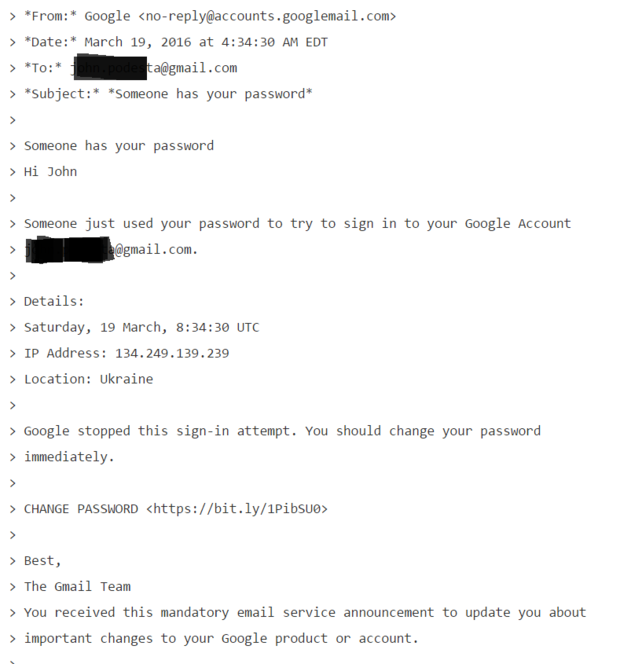
\includegraphics[scale=0.7]{{./section1/podesta.png}}
    \caption[Phishing email sent to John Podesta]{Phishing email sent to John Podesta}
    \label{fig:Podesta}
\end{figure}

Successful phishing attacks are expensive to organizations. In 2020 alone, phishing attacks cost US businesses more than \$1.8 billion, up from \$1.7 billion in 2019 \cite{vade}. These attacks can lead to credential/account compromise, giving the attacker access to sensitive information, et cetera. Attackers may try to use these data for extortion. For example: In 2014, an attack was successful on an invasion of celebrity iCloud accounts, leading to the leaking of nude photos. The leak was initially considered due to a breach on Apple services, but it was a phishing attack. The attackers pretended to be Apple and Google and asked users to change their password \cite{duke_2014, guardian_2014}.

Phishing attacks are continuously rising and have doubled since early 2020. In July 2021 alone, the Anti-Phishing Working Group (APWG), an international consortium that attempts to eliminate fraud and identity theft caused by phishing, saw 260,642 phishing attacks \cite{apwg}. Additionally, Proofpoint, a security enterprise that provides cybersecurity products relating to emails and digital information, found that more than 75\% of organizations faced phishing attacks in 2021 \cite{proofpoint}. These uprising trends in phishing attacks have shown some serious need for mitigations.

\section{Current Mitigations}
The prevention of phishing attacks can be divided into three steps \cite{vayansky}—the first step is preventing the attack from reaching the end-user. We have seen multiple studies on phishing prevention with the help of the machine learning models \cite{yang_zheng_wu_wu_wang_2021, sahingoz_buber_demir_diri_2019}. Machine learning approaches such as K-nearest, XGBoost, CNN, RCNN, Random forest, et cetera. are commonly used to detect patterns and generalize phishing attacks. Some of the models have shown promises with more than 90\% accuracy—however, a study conducted by What.Hack has shown that only one of the ten anti-phishing tools tested could correctly identify over 90\% of phishing websites. That tool also incorrectly identified 42\% of legitimate websites as fraudulent \cite{what_hack}. Moreover, attackers are always looking for the best way to bypass these automated systems and develop new techniques. The evolving nature of phishing attacks calls for an additional layer of security on top of the prevention layer.

If the attacks reach the user, the next step to secure the user is by warning them. Most modern web browsers and email clients warn users of any suspicious activities they detect. For example, the browser actively warns users with pop up for probable phishing sites. In addition, browsers provide passive hints to understand URLs better. Browsers use different shades of white to inform the user about a "fully qualified domain name (FQDN)" (also called absolute domain name), the complete domain name for a specific host on the internet. Figure \ref*{fig:browser_cues} shows a use case for such a hint. Attackers will intentionally have a confusing link to trick users into clicking the link. For example, although "help.google.com.bubble.com/changepassword" seems like an email from Google, the actual domain is bubble.com. The domain owner can add any subdomain to domains they own, such as help.google.com.bubble.com, which can potentially be used in phishing attacks. Modern email clients provide similar hints for spam emails and notify the users if they can not verify the sender. Active warnings are more effective than passive signs \cite{vayansky}. Still, attackers can easily bypass these warnings by creating new sites and context-aware websites or emails every time they are flagged.

\begin{figure}[h]
    \centering
    
\includegraphics[scale=0.7]{{./section1/browser_cues.png}}
    \caption[Browser cues on links]{Browsers uses different shades to indicate the primary link.}
    \label{fig:browser_cues}
\end{figure}

The final step to avoid phishing emails is user training. A study done by Proofpoint shows that 34\% of US respondents believe emails with familiar logos are safe \cite{proofpoint}. The study indicates a general lack of awareness about phishing campaigns among the general population. As emails are the most frequent phishing attacks, many phishing training focuses on training users to detect phishing emails. Our gameplay will focus on emails to train the users against phishing attacks.

One of the most common tools to train users is cyber security videos and reading materials. However,  Kumaraguru et al. saw that users seldom seek these materials and tend to ignore emails directing them to these materials \cite{johnny_phishing}. In addition, they noticed that most users do not spend much time reading security-related tutorials. This calls for an interactive training program to keep the user focused and engaged during training.

We have seen new and existing training materials incorporating gaming techniques. Gamification has been gaining rapid popularity over the past decade\cite{schultz_2021}. It increases engagement by incentivizing learners to pay attention and complete activities. We can observe existing training videos incorporating gaming techniques, such as letting users choose the correct option in the middle of training videos (a mini quiz game) and giving badges after completion. Newer training videos take gamification further and let learners play through various scenarios, make choices and see the rewards or consequences of their decision. For example, "Infosec's Choose Your Own Adventure Security Awareness" Game\cite{infosec_2022} has interactive storytelling to keep the user focused till the end of the video.

Gamification has improved the interactivity with the user, but existing training videos fail to cover the technical details that are commonly found in phishing emails. Our gameplay covers various technical aspects commonly found in phishing emails, such as domains, spoofing, and link hiding techniques attackers use to trick users.

\section{Litearature Review}

\subsection{Serious games}
Gaming approaches in education have been used for over a decade\cite{almeida_2012}. There is a dedicated genre of games (typically online applications), termed serious games. These games communicate specific information that helps introduce relevant concepts and apply those concepts to solve problems. The primary purpose of these games is to promote learning alongside entertainment. With the help of different game design techniques (rewards, story progression, feedback systems), users are more engaged and immersed while learning. In addition, the virtual world also provides users with a safe space to experiment without real-life consequences.

Serious games are used in many fields such as education, healthcare, and training. For example, "Garfield's Count Me In" \cite{count_me_in} helps children in (special education) primary school practice their arithmetic skills. This math game contains different exercises or 'brick,' which form the foundation for a new layer of exercises. The game design help students master the first layer of exercises before moving to the next layer (basic to advanced).

"Killer Flu" \cite{killer_flu} (one of many games by "Persuasive Games") is another example of a serious game that attempts to explain how flu mutates and spreads and how challenging it can be for a deadly strain to affect a large population geographically. The game helps spread awareness by making the player take the role of the flu itself, trying to mutate and then spread it in various conditions. Serious games (such as Killer Flu) can place the user as any character in the game to get the idea across. We use a similar concept in our game by placing the player as the attacker (rather than the victim as many existing training materials do.)


\begin{figure}[h]
    \centering
    \begin{minipage}{0.49\textwidth}
        \centering
        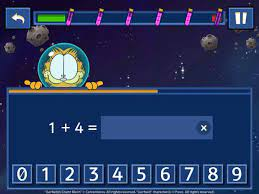
\includegraphics[width=0.9\textwidth]{./section1/garfield.jpeg}
        \caption{Garfield's Count Me In}
    \end{minipage} \hfill
    \begin{minipage}{0.49\textwidth}
        \centering
        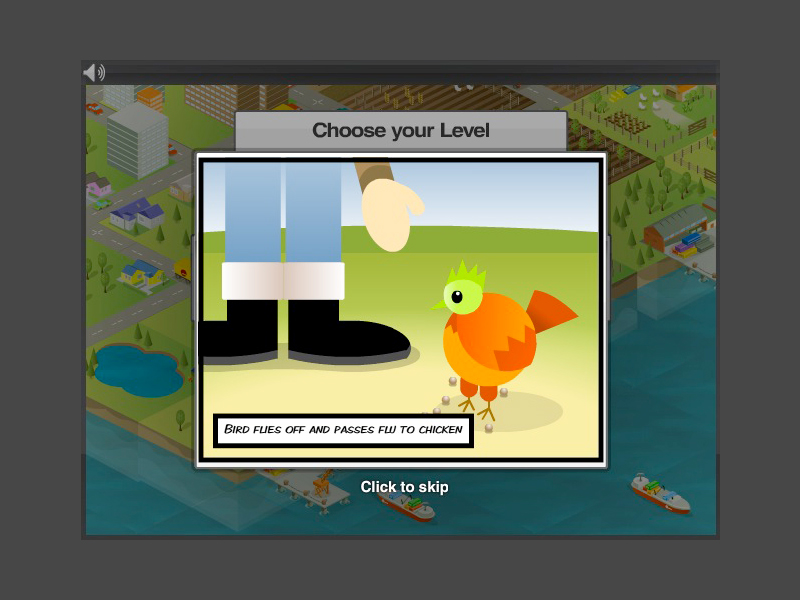
\includegraphics[width=0.9\textwidth]{./section1/killer_flu.jpg}
        \caption{Killer Flu}
    \end{minipage} \hfill
\end{figure}

There have been various studies about using games as a practical phishing training module. Hendrix et al. \cite{hendrix_al_sherbaz_bloom_2016} compared the effectiveness of cyber security training tools with some popular games designed for cyber security training. They found that existing games, in general, had a positive impact on learning, with positive education experience.

We can broadly classify current training games into three main categories. We discuss each of these categories and provide some examples of each type in the following sections.

\subsection{Board and card games}
There have been studies based on non-computer-based games. For example, Control-Alt-Hack \cite{control_alt_hack} and "smells phishy" \cite{smels_phishy} are card games aimed to train users against phishing. Both the games show promise in their approaches and teach the user what to be aware of (such as spelling mistakes, phishing links) through their gameplay. After playing the game, users reported higher efficiency and ability to detect phishing emails.

Although both the games show promise in their approach, non-computer-based games have some inherent limitations. The games have a barrier of entry as it requires pre-setup (with the need for the cards and boards). Furthermore, once the games are deployed, they are permanent, limiting their ability to train and evolve against new phishing attacks. Finally, board and card games fail to communicate the context of the attack and lack examples of where they might be used. For example, although the game might have a "hiding links" card, the users lack knowledge on how and when it might be used. The limited skills these games provide may not be best suited as an individual training module.

\subsection{Phishing Link (URL) training}
There have been numerous computer games about phishing. However, many studies focus on one common category: training users to verify phishing links. Anti-Phishing Phil \cite{anti_phishing_phil} is one of the pioneers in this field. Their gameplay puts the user as a fish. The goal of the fish is to grow larger by eating the good bugs (non-phishing links) and avoiding the bait (phishing links). The game has four different levels, with each round focusing on another type of deceptive URL. Players move to the next level after correctly identifying six out of eight URLs.

There are other similar games to Anti-Phishing Phil. For example, Phish Phinder \cite{phish_phinder} builds upon the Anti-Phishing Phil storyline and game design. However, it differentiates itself from Anti-Phishing Phil by integrating self-efficacy in the game design to enhance phishing avoidance motivation and behavior among users. They were able to positively impact self-efficacy by adding conceptual knowledge (through challenges) and procedural knowledge (through increasing levels and repetition of conceptual knowledge).

"Building Confidence not to be Phished"\cite{gamified_approach} by Baral et al. developed a game prototype aimed to enhance an individual's self-efficacy in phishing threat avoidance. They developed a ballon shooter game where the main character has to shoot balloons with legitimate URLs (similar to previous games). Although the links and hints are displayed in a different context, this game tries to achieve the same goal as previous games.

All these games have one thing in common: they teach users how to identify legitimate URLs through their gameplay. As URLs are one of the most critical factors while detecting phishing emails, gameplay dedicated to recognizing phishing URLs serves as a suitable training module. Anti-Phishing Phil results show that their game has a good impact compared to existing training material to differentiate legitimate links from phishing links.

However, these games might not be suitable as standalone training against phishing. Although URL training games are a sound training module, these games fail to train users on some common tricks seen in phishing attacks. For example, one of the most significant limitations of these games is the lack of context on where the link might appear. As such, attackers can use different link hiding techniques to trick the user into clicking the link. Moreover, attackers use psychological manipulation to trick users into clicking the link by creating a sense of urgency, fake giveaways, or making it seem like an email from somebody individuals know to trick people into clicking the link.

\subsection{Role playing game}
"What.Hack" \cite{what_hack} saw the shortcomings of the link-based game and developed gameplay that train the user on links as well as email context. It puts the user as a bank employee required to process emails to acquire contracts and protect their network from cybercriminals. The game approaches the training by having the user role play as a victim and looking at different techniques found in actual attacks. The game's goal is to block phishing attempts and allow legitimate emails. It simulates the harmful effects of phishing by "firing" the employee in-game if they allow too many phishing emails, take too long, or misclassify a significant number of legitimate emails as phishing emails.

\begin{figure}[h]
    \centering
    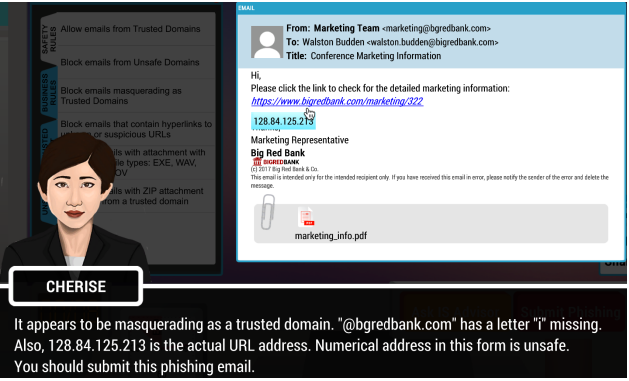
\includegraphics[width=0.9\textwidth]{./section1/what_hack.png}
    \caption{What.Hack gameplay}
\end{figure}

"What.Hack" gameplay incorporates previous studies' different techniques and builds upon them. In addition, its context-based email training module solves one of the drawbacks of link-based training games. Since players are looking at full emails (both phishing and legitimate) obtained from the real world, users can better recognize the context of the email and what to look out for in emails to stay protected. Moreover, the emails generated in this game successfully incorporate the objective of primary link-based game goals.

The result from "What.Hack" shows clear improvement regarding link-based games. In comparison to Anti-Phishing Phil, "What.Hack" improved players correctness in identifying phishing emails by 36.7\% \cite{what_hack}.

\section{Objective}

"What.Hack" clearly demonstrated that role-playing games with contextual emails were more effective than existing gameplays. Unfortunately, we could not find any other significant study that tried to build upon this finding. Therefore, we have developed gameplay inspired by "What.Hack" but approached the role-playing aspect as an attacker instead of a victim.

Current phishing training programs focus on training the user as a victim. Our game tries to approach training from a new direction by placing the player as an attacker. This approach will let the users see what the phisher might concentrate on while creating a phishing email and, in turn, use that knowledge to detect phishing emails. The training objective of our game is similar to exisiting games and tries to build upon it. Table \ref{tab:game-type} compares the main training objective of our game with existing games.

\begin{table}[!ht]
    \resizebox{\textwidth}{!}{%
        \addtolength{\tabcolsep}{-10pt}
        \begin{tabular}{p{0.13\textwidth} p{0.48\textwidth} l l l}
            \hline
            \textbf{Game Type}   & \textbf{Description}                                                                                 & \textbf{URL}          & \textbf{Spear} & \textbf{Spoof} \\
            \hline
            \textbf{Link Based } & Teach users to differentiate phishing links from non-phishing links                                  & \centering \checkmark &                &                \\

            \textbf{Board Game}  & Teach users high- level security concepts                                                            & \checkmark            & \checkmark     & \checkmark     \\
            \textbf{What.Hack}   & Teach players to defend against phishing attempts in realistic simulation game (playing as a victim) & \checkmark            & \checkmark     &                \\
            \textbf{Our Game}    & Teach players to recognize and defend against phishing attempts by role playinig as a victim         & \checkmark            & \checkmark     &                \\
            \hline
        \end{tabular}%
        \addtolength{\tabcolsep}{10pt}
    }

    \caption{Different type of training games and their main objectives}
    \label{tab:game-type}
\end{table}

Our goals for the study can be summarized as:

\begin{itemize}
    \item We designed and developed a phishing training game that attempts to incorporate the objectives of the current existing games and build upon them. Our game includes link hiding training and provides context to those links.
    \item We compare the participants' performance before and after playing the game. We evaluate users' results and try to understand user thought processes behind each decision.
    \item Finally, we list some of the insights found during the survey and list potential mitigation and training.
\end{itemize}




%%%%%%%%%%%%%%%%%%%%%%%%%%%%%%%%%%%%%%%%%%%%%%%%%%%%%%%%%%%%%%%%%%%%%%%
%%%                           System Description
%%%%%%%%%%%%%%%%%%%%%%%%%%%%%%%%%%%%%%%%%%%%%%%%%%%%%%%%%%%%%%%%%%%%%%





\chapter{System Description}

This chapter will discuss our current game design, the story, mechanics, and tools used, and briefly discuss the previous iterations of the game.

\section{Game Description}
The game is developed on React\footnote{\url{https://reactjs.org/}} with Chakra UI\footnote{\url{https://chakra-ui.com}}. We use Supabase\footnote{\url{https://supabase.com/}} to keep logs of user interaction with the game. Figure \ref{fig:screenshot} shows the initial state of the game.

\begin{figure}[h]
    \centering
    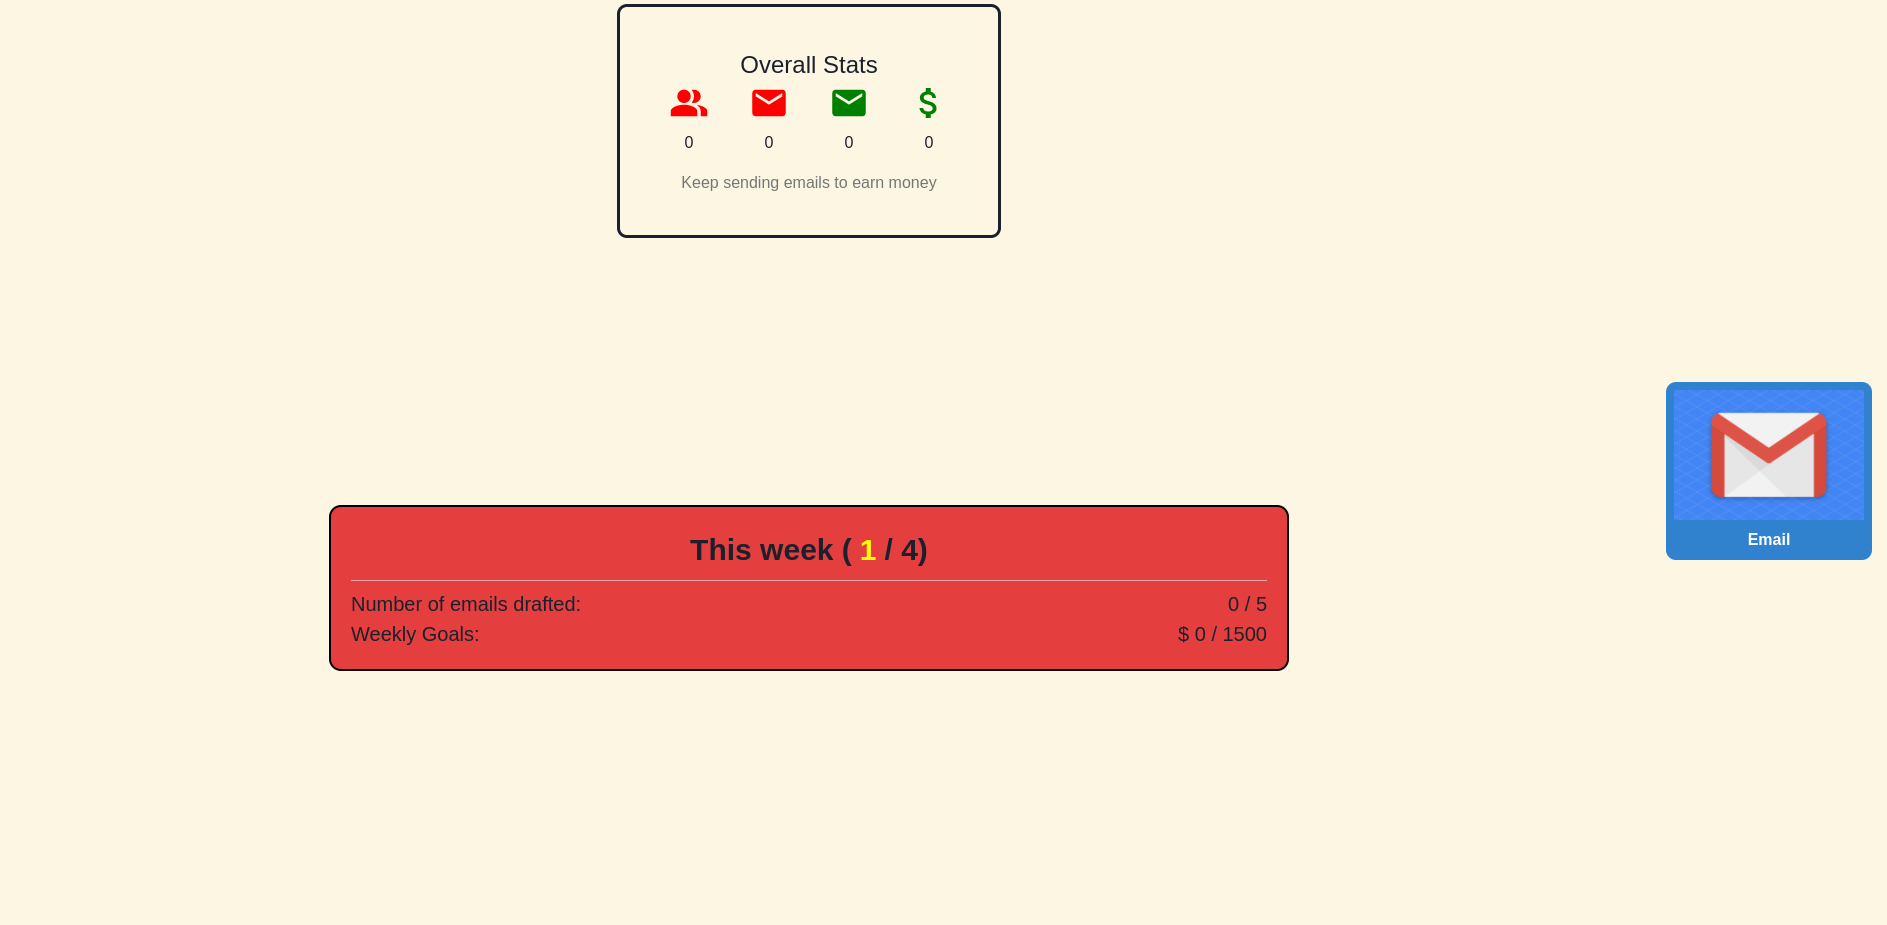
\includegraphics[width=\textwidth]{figures/section2/game.png}
    \caption{Screenshot of initial state of the game}
    \label{fig:screenshot}
\end{figure}

\subsection{Game Story}
The game's main character has taken a large loan from a loan shark. The goal of the game is to pay off the loan in time. However, as the loan is substantial, he cannot earn enough money through hard work and uses phishing tricks to scam people. However, the main character does not know the intricacies of sending out phishing emails himself, so he hires a helper to create phishing emails. Together, they have decided to impersonate PayPal. The player has four weeks to earn enough money to pay back.

\section{Mechanics}
Our main objective while developing the game was to streamline the player experience and ensure players would be exposed to the maximal variety of phishing techniques included in the game. Unfortunately, our initial iteration of the game prevented us from making sure that players looked at all the techniques in the game and played them to maximize the game learning objective. We will discuss the previous iteration's limitations in detail in a later section and concentrate on the current iteration for now.

We divided the game into four weeks (parts) to streamline the game and make sure players looked at each objective. Each week's progression will unlock specific skills users' can use to create an email. We will discuss specific week progression and how it ties the game together in later sections.

\subsection{Components}
Before we deep dive into the game's flow, we have to discuss individual components. At the top level, we can divide the game into three components: attacker, marketplace, and email generation.

\subsubsection{Atttacker}
The attacker module handles training the helper with available skills. There are six different skills that the player can train the helper on, each corresponding to techniques and qualities present in real-world phishing attempts, namely spelling, grammar, styling, links, spoofing, and research. We divide these skills into language skills (spelling and grammar) and technical skills (styling, links, spoofing, research). Language skills are passive skills in the game, whereas technical skills, except for styling, are active skills.

Training on passive skills will improve the quality of all subsequent emails generated by the helper without additional input from the player. In contrast, active skills unlock additional choices for the player to make when composing subsequent emails. For example, after the player trains their helper on spelling, the attacker will stop making spelling errors without additional feedback from the user. Training the helper on links will give the user different options to hide the links while creating the email. Table \ref{tab: attacker} lists the skills and their effect in the game in brief. We will talk about the different properties activated by each skill in the email generation section.

\begin{table}[!ht]
    \centering
    \resizebox{\textwidth}{!}{%
        \begin{tabular}{p{0.05\textwidth} p{0.05\textwidth}  p{0.05\textwidth}  p{0.5\textwidth}}
            \hline
            \textbf{Skills} & \textbf{Active/} & \textbf{Cost} & \textbf{Effect}                                                   \\
                            & \textbf{Passive} &               &                                                                   \\
            \hline
            Spelling        & Passive          & 1,000         & Creates emails without spelling errors                            \\
            Grammar         & Passive          & 1,000         & Create emails without grammar errors                              \\
            Styling         & Passive          & 2,000         & Create stylized emails with better header, footer, and images     \\
            Links           & Active           & 3,000         & Unlocks different techniques to hide the link while sending email \\
            Research        & Active           & 3,000         & Gives the user option to generated targeted emails                \\
            Spoofing        & Active           & 4,000         & Gives the user ability to spoof the email                         \\
            \hline
        \end{tabular}%
    }
    \caption{Different skills and their effect in the game}
    \label{tab: attacker}
\end{table}

We chose the skills in the game to replicate the training objective of existing training modules and common properties found in phishing emails. Each skill in the game has a training cost associated with it. We associated some costs with skills to represent training requires some resources. The cost is kept at a minimum to let the user unlock it as soon as possible but scaled such that more efficient skills have a higher price than general skills. Keeping the cost low allowed the user to focus more on using those skills to generate emails rather than earning money to train attackers.

\begin{figure}[!ht]
    \centering
    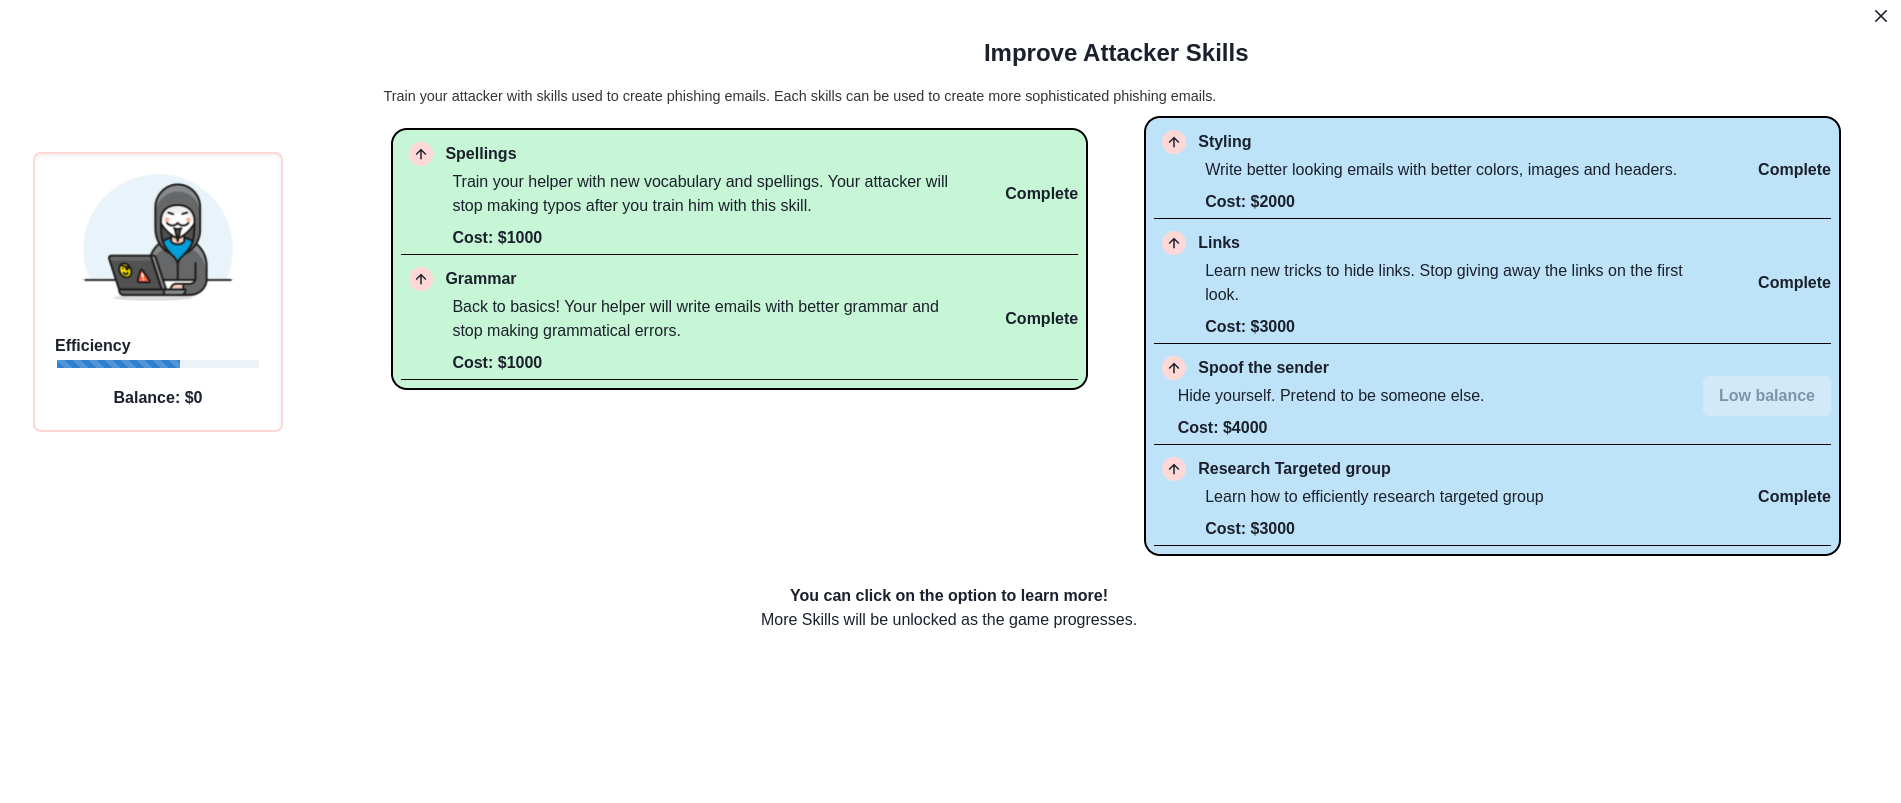
\includegraphics[width=\textwidth]{figures/section2/attacker.png}
    \caption[Screenshot of the attacker module on week 4]{The screenshot shows different skills available to the player in week 4. Trained skills are displayed as Complete, whereas skills that can be trained are displayed as "Train."}
    \label{fig:attacker}
\end{figure}

Although we tried to include all the common properties found in phishing emails, we could not itemize some general properties such as sense of urgency, generic greetings, too good to be true emails, et cetera. Therefore, instead of itemizing and adding more passive skills, we decided to limit the number of skills and let users actively concentrate on those. On the technical side, the limited number of properties to look at while generating emails made email generation much more manageable and allowed us to generate a broader range of emails. In addition, exposing players to more phishing emails may help players recognize similar emails and patterns later.

Current emails generated by the system still include the properties of phishing emails that we could not itemize. For example, generated emails might have a sense of urgency, but the player cannot actively select this option.

\subsubsection{Marketplace}
The marketplace allows the player to purchase domains to use while generating emails (See figure \ref{fig:marketplace}). Existing training modules train the players to recognize phishing links (which are generated by the system) but do not allow players to try custom domains. In our gameplay, the attacker "Link" skill teaches how phishing emails hide links to trick victims into clicking the link.

\begin{figure}[!ht]
    \centering
    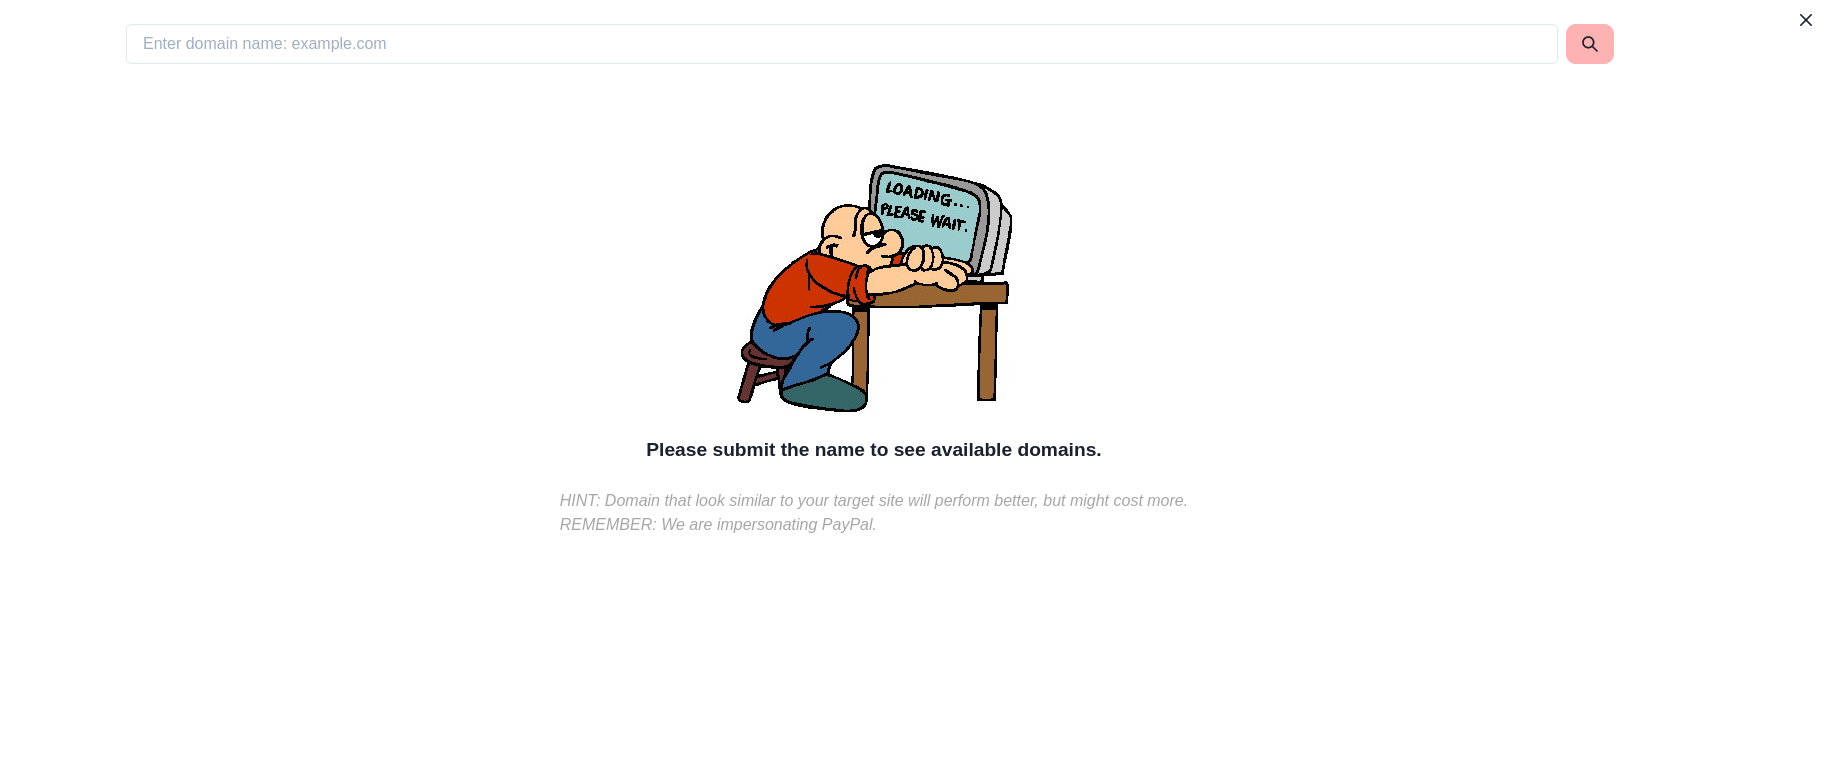
\includegraphics[width=1\textwidth]{figures/section2/marketplace_empty.png}
    \caption[Screenshot of marketplace]{The marketplace accepts any valid domain name}
    \label{fig:marketplace}
\end{figure}

The first step when letting the user purchase a domain is to check if the domain is valid. A valid domain is a second-level domain followed by a top-level domain in our game. A top-level domain refers to the last segment of a domain name, and a second-level domain refers to the name just to the left of the top-level domain. For example, "test.com" is a valid domain where "test" is a second-level domain and "com" is the top-level domain. We validate the second-level domain with the help of the following regex code:

\hfill
\begin{lstlisting}[basicstyle=\small]
    if (userLink.includes(" ") || !/^[a-zA-Z0-9-.]*$/.test(userLink))
        return;
\end{lstlisting}

We do not allow special characters (Fada Accent) in the domain name for simplicity.

Over 1,500 top-level domains (TLDs) are currently used in the web  \cite{tld}. For simplicity, we only allow users to choose from a predefined list filtered from Tranco list \cite{trancos} which provides us with the most popular one million domains, similar to Alexa top site. We filtered top-level domains that occurred at least a hundred times from Tranco's list and got 262 TLDs. This limited number of top-level domains allowed us to incorporate commonly used TLDs while ensuring the game did not have a large processing time while purchasing domains.

\begin{figure}[h]
    \centering
    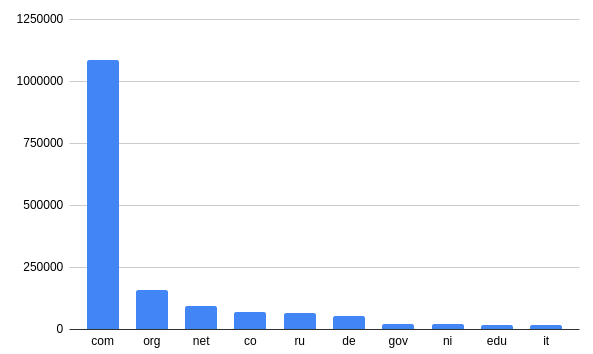
\includegraphics[width=0.7\textwidth]{figures/section2/tld.png}
    \caption{Top 10 top level domains present Tranco list}
    \label{fig:marketplace_tld}
\end{figure}

Players can choose any combination of valid characters for the second-level domain (validated by the regex pattern shown above). For example, "123test.com" is a valid domain. However, "\%ssda1.com" is not a valid domain. We maintain the top 1000 domains in the Tranco list to prevent purchasing popular and already existing domains. This list consists of popular sites such as "google.com," "facebook.com," "netflix.com," including "paypal.com" (which is used by our game to train the user). We had to trim the number of domains to a thousand as processing a million domains required significant processing time, impacting the gameplay. Since the number of domains is limited, some popular sites such as "uno.edu," "messenger.com," "bitbucket.org," et cetera, are still available.

In the game, players are explicitly asked to impersonate PayPal to trick the victims, so domains closer to PayPal will perform better. Like the real world, purchasing a new domain requires in-game currency -- the same currency user use to pay off their loan. Thus, users are incentivized to purchase inexpensive domains to pay off their loans while also considering that domains that look more similar to what they are impersonating (here, PayPal.com) are more likely to trick more users.

Although, the game focuses on PayPal, domains similar other popular services also has a higher cost. The list of popular services is obtained from Tranco list (as discussed above) for our game. Since the user can purchase any domain and domains closer to the top thousand domains are more expensive,  the cost of a domain does not directly correlate to higher efficiency in the game.

We determine the closeness between two domains based on string similarity. We use Sørensen-Dice coefficient to compute the similarity between two strings. Mathematically, given two sets, X and Y, we can define Dice coefficient as:

\begin{center}
    \begin{math}
        DSC = \frac{2|X \cap Y|}{|X|+|Y|}
    \end{math}
\end{center}

It produces a value between zero and one, making the cost calculation of domains much easier. Table \ref{tab:dice} shows examples of some custom domains along with their similarity. We can see that a domain similar to "paypal" has a higher similarity. Therefore, we treat domains with higher similarity score as more efficient for our game. We do not use the top-level domain for cost calculation, as most players usually choose ".com," which impacts the string similarity.

\begin{table}[!ht]
    \centering
    \begin{tabular}{r|l}
        \textbf{Custom Domain} & \textbf{Similarity with "paypal"} \\
        \hline
        paypale                & 0.90                              \\
        palpay                 & 0.80                              \\
        paypl                  & 0.66                              \\
        appl                   & 0                                 \\
        test                   & 0                                 \\
    \end{tabular}
    \caption{Different second level domain and their similarity with "paypal"}
    \label{tab:dice}
\end{table}

The cost of the domain does not depend solely on similarity to "paypal". While calculating the cost, we get the maximum similarity with any of the domains in the top-1000 list. If the similarity with the existing domains is below 0.6, we assign a base price of 500 for the domain; else, the general cost of the domain is calculated as:
\begin{center}
    \begin{math}
        cost = 500 + (similarity *100)^2 * 0.56
    \end{math}
\end{center}

If the player tries to buy existing domain, the game suggests domains ending with alternate top level domains (See figure \ref{subfig:marketplace-unavailable}). For example, if the player tries to buy "paypal.com", the game suggests top 10 alternate top level domains such as "paypal.org" or "paypal.net". The cost of such domain is not based on similarity. We use the frequency of top level domains in Tranco list and compute the cost as follows:

\begin{center}
    \begin{math}
        cost = (50 * \sqrt{10-index}) *25
    \end{math}
    \text{where index is the ranking of the top level domain based on frequency in Tranco list.}
\end{center}

\begin{figure}[!ht]
    \centering
    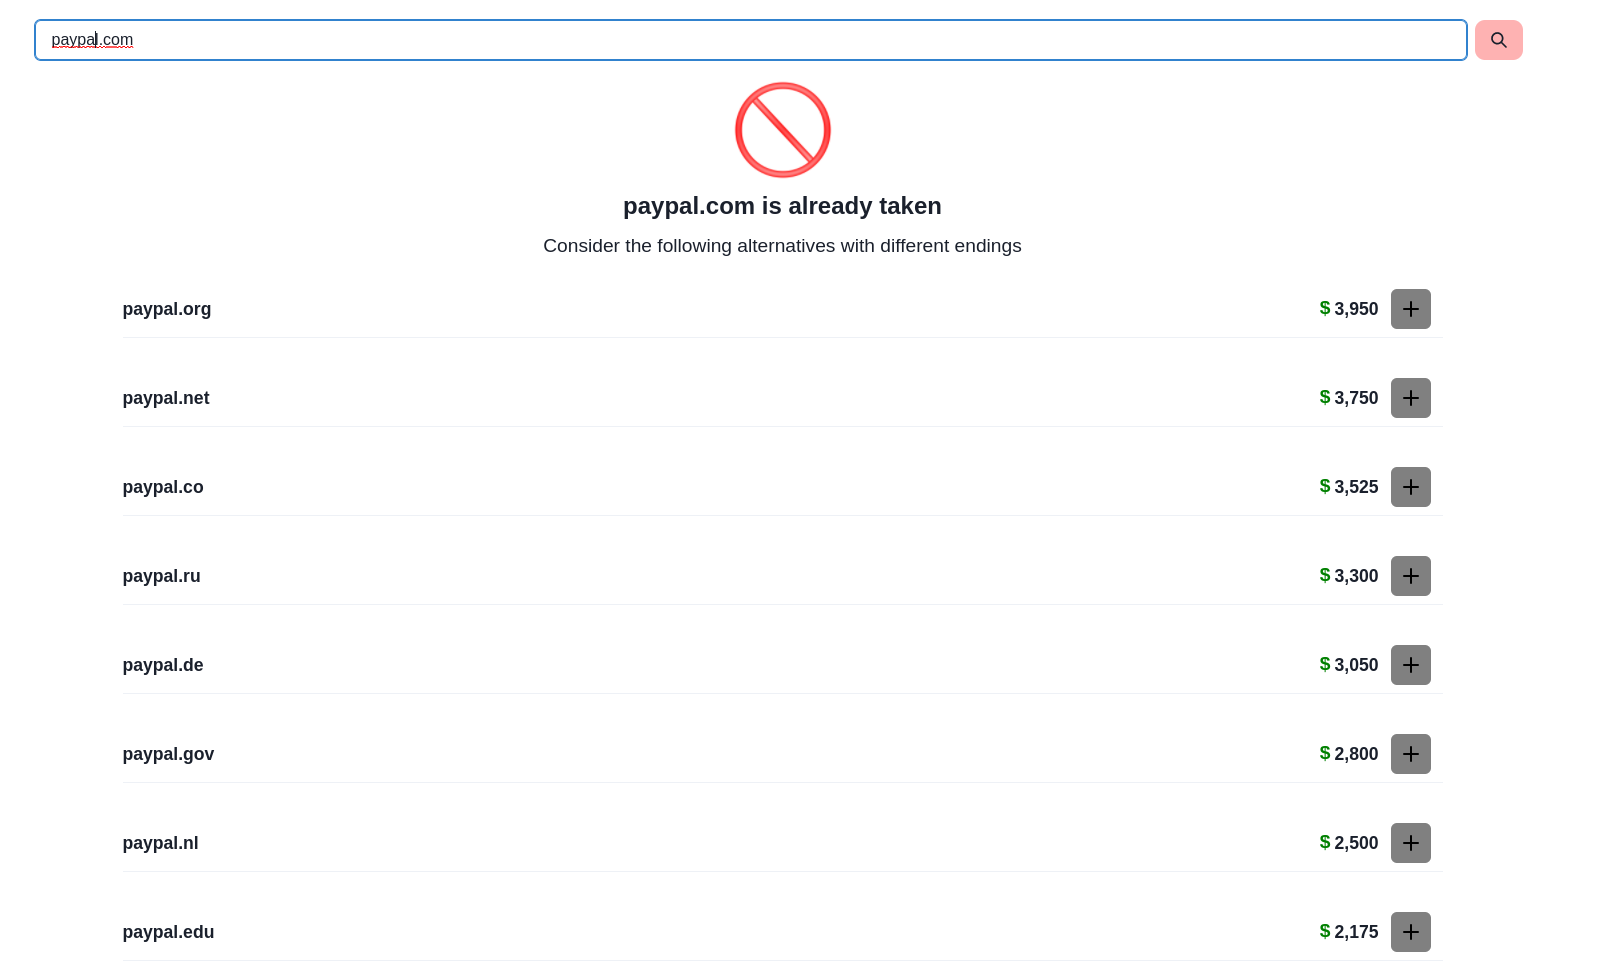
\includegraphics[width=\textwidth]{figures/section2/marketplace_unavailable.png}
    \caption[Marketplace unavailable]{Marketplace unavailable. The game gives different alternatives if the user tries to buy an existing domain. For example, if the user tries to buy "paypal.com", the game suggests top 10 alternate top level domains such as "paypal.org" or "paypal.net".}
    \label{subfig:marketplace-unavailable}
\end{figure}

\begin{figure}[!ht]
    \centering
    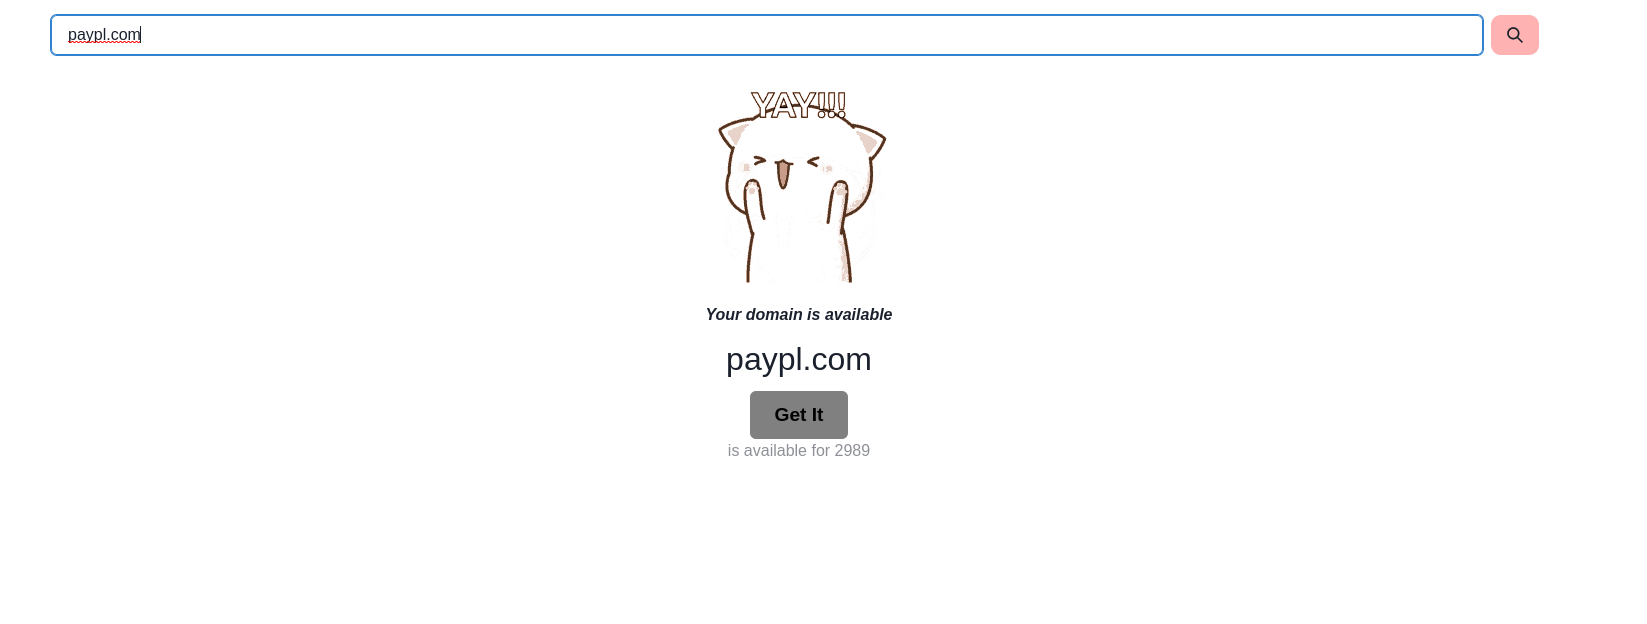
\includegraphics[width=\textwidth]{figures/section2/marketplace_available.png}
    \caption[Marketplace available]{Marketplace available. Screenshot of the marketplace when domain selected by the user is available. (paypl.com in the screenshot) }
    \label{subfig:marketplace-available}
\end{figure}


\begin{figure}[!ht]
    \centering
    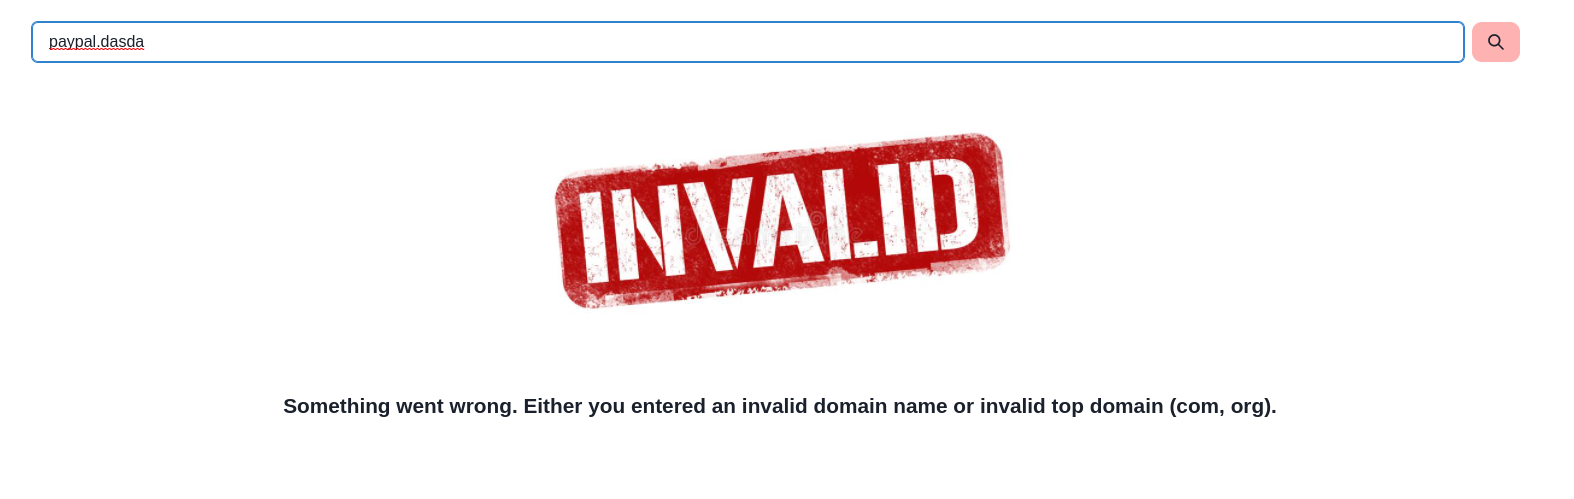
\includegraphics[width=\textwidth]{figures/section2/marketplace_invalid.png}
    \caption[Marketplace available]{Screenshot of the game when user enters invalid characters or TLDs. In this example, "dasda" is an invalid TLD.}
    \label{subfig:marketplace-invalid}
\end{figure}


These formulas to calculate cost are not standard and were achieved through trial and error. Although not an actual scale, we set the cost to show that domains closer to real-world domains will have a higher cost.
% with changes to game, we changed the scale to make it achievable

\subsubsection{Emails}
The emails component ties up the game by generating and sending emails based on attacker skills and the current domain. The system randomly chooses an email from 30 available emails based on the user input (active and passive skills). These emails were handpicked to replicate real-life phishing attempts. We chose emails that were most common during our initial Google search. To ensure we did not miss any common phishing emails, we read multiple blogs and added common phishing emails and patterns found in them. As a result, emails in the system include common phishing tricks used by attackers and various emails such as log-in emails, welcome emails, limited account emails (emails when services limit your account while waiting for additional information), et cetera.

Before discussing sending email and efficiency, let us discuss how each skill impacts the email generation process. As mentioned in the attacker component section, passive skill does not require additional input from the player and improves the generated email after training them. Spelling, grammar, and styling in our game fall under passive skills. Before players train on spelling and grammar, they will be required to recognize spelling and grammar errors. We wanted to point out spelling and grammar errors as they are commonly found in poorly worded phishing emails and are recognized as one of the common ways to differentiate phishing emails from legitimate emails. However, we do not want users to spend all their time finding language errors, so we generate proper grammar and spelling emails after players train on them. Figure \ref{subfig:passive-untrained} shows an example of an email generated by the game before players train on spelling and grammar.

\begin{figure}[!ht]
    \centering
    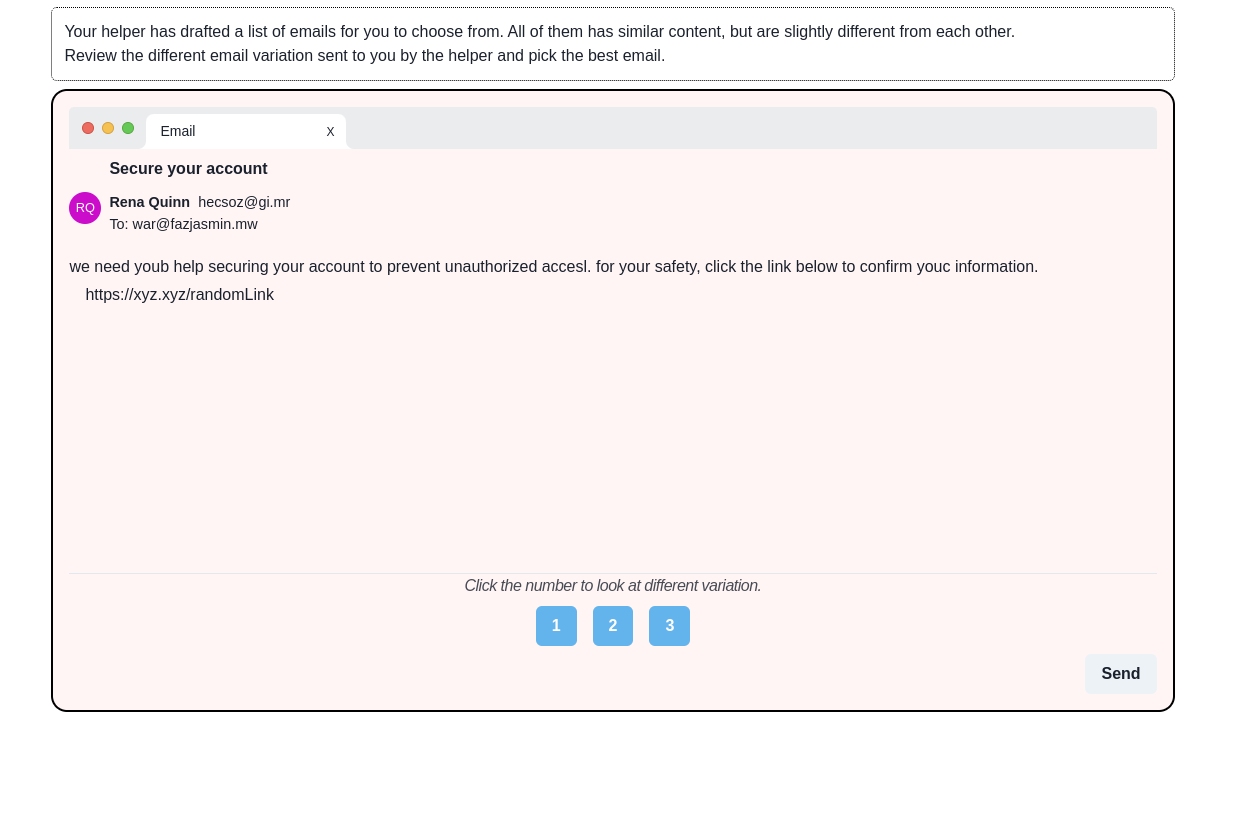
\includegraphics[width=\textwidth]{figures/section2/passive_untrained.png}
    \caption{Emails generated before training on passive skills contains spelling and grammar error with no styling (contains text only)}
    \label{subfig:passive-untrained}
\end{figure}

Styling increases the visual appeal of the email with the help of images, header, footer, and better styles. Emails sent by an organization generally contain images and styling. Attackers use this fact to trick victims by including company logos and images. As stated before, users generally trust familiar logos and 34\% of users believe emails with familiar logos are safe \cite{proofpoint}. Figure \ref{subfig:passive-trained} shows an example of an email generated by the game after players train on spelling and grammar with styling.

\begin{figure}[!ht]
    \centering
    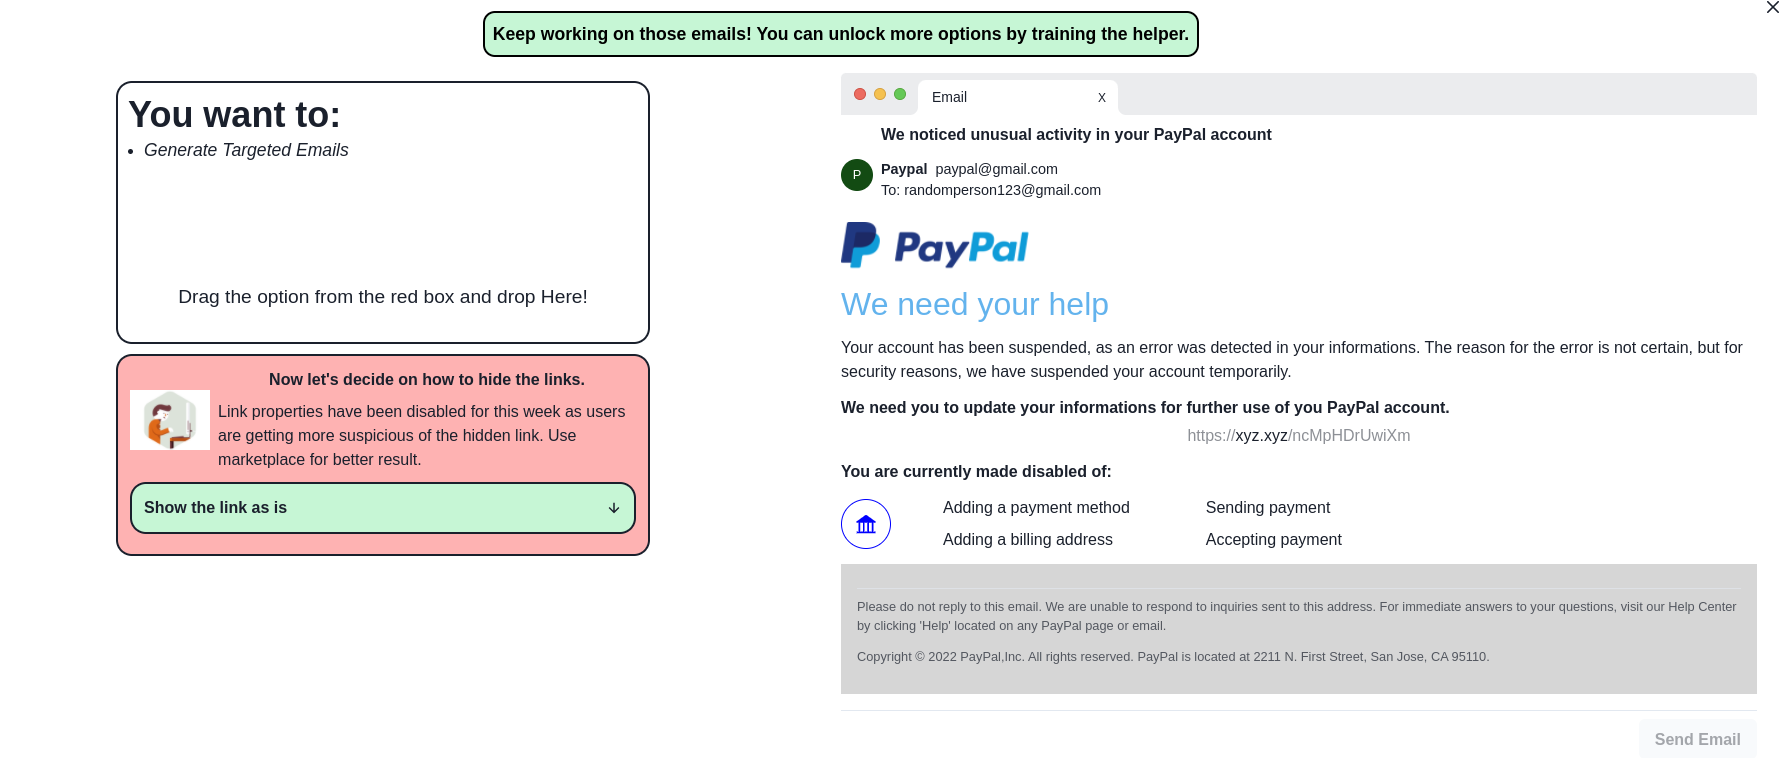
\includegraphics[width=\textwidth]{figures/section2/passive_trained.png}
    \caption{Emails generated after training on passive skills generate emails with proper grammar and spelling with styling}
    \label{subfig:passive-trained}
\end{figure}

Active skills give the user more options to fine-tune the generated email. Our game's active skills are links, research, and spoofing. Each option allows the user to modify a part of the generated email. We discuss each of these skills in detail below.

Research skill allows the player to generate targeted emails. Before training on research, the helper only generates a generic email, and players do not get an option to send targeted emails. Generic emails target a larger audience and do not contain specific user details. On the other hand, targeted emails contain user-specific information such as address and name. With this skill, we wanted to replicate spear phishing, a phishing method that targets specific individuals or groups within an organization. Figure \ref{fig:targeted} shows an example of a targeted email generated by the game.

\begin{figure}[ht]
    \centering
    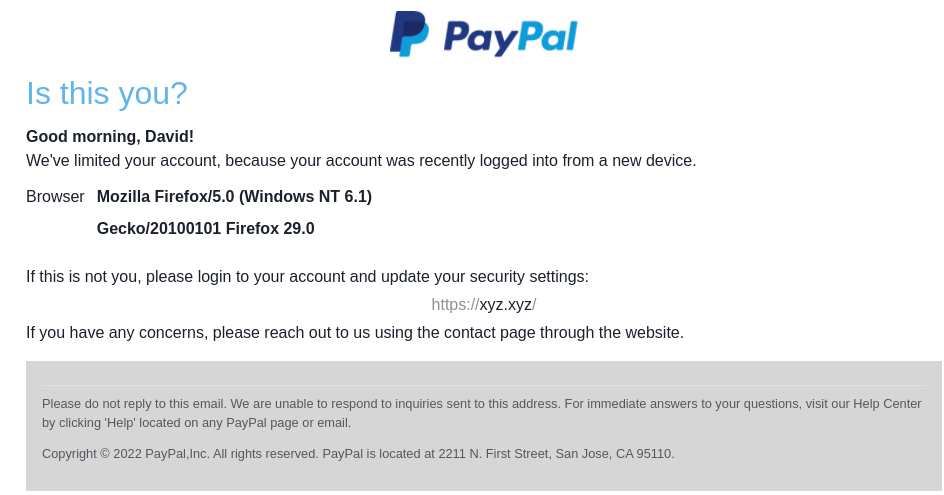
\includegraphics[width=0.9\textwidth]{section2/targeted.png}
    \caption{Example of a targeted email generated by the system}
    \label{fig:targeted}
\end{figure}

All the emails on the system are pre-labeled to either generic or targeted. When the user chooses an option, the system will filter out emails (based on user option) and randomly choose an email from the filtered list.

Our second active skill, links, attempts to cover URL/link training many current phishing training games covers. Training the helper on link unlocks different ways to display the link when generating an email. We chose these options after reviewing real-world phishing emails and current training materials.

The game allows the user four different ways to display the link:

\begin{enumerate}
    \item \textbf{Hide under button or text}\\
          One common phishing trick is to hide the actual link behind some text or button. We replicate this behavior with our "Hide link" option, which displays some text or buttons as links without displaying the actual link. To familiarize users with different forms of text messages and buttons, we randomly choose a text message (Example figure \ref{fig:hide-text}) or button (Example figure \ref{fig:hide-button}) from a predefined set of input. Our input contains familiar texts such as "Click here," "Go to PayPal," "www.paypal.com/help," and other similar alternatives. Players can hover over the text or button to visualize the link (similar to real email clients).

          \begin{figure}[!ht]
              \centering
              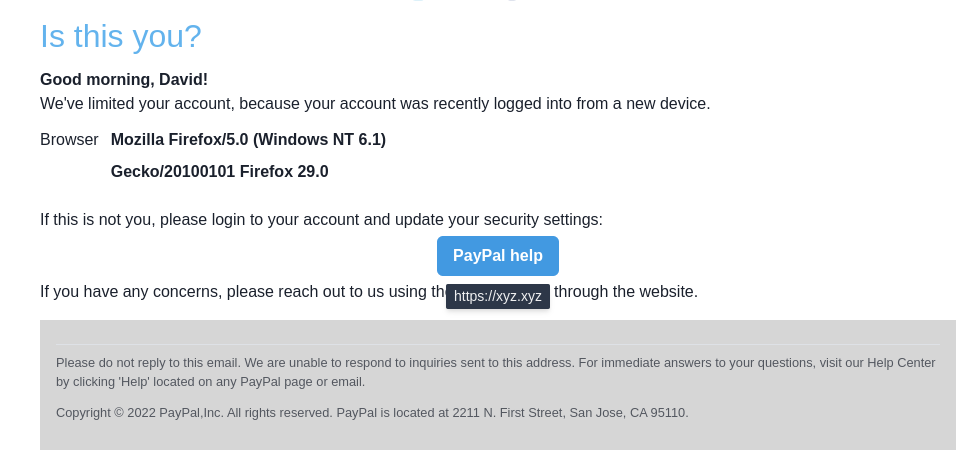
\includegraphics[width=\textwidth]{figures/section2/hide_button.png}
              \caption{The actual link is hidden behind the button}
              \label{fig:hide-button}
          \end{figure}

          \begin{figure}[!ht]{
                  \centering
                  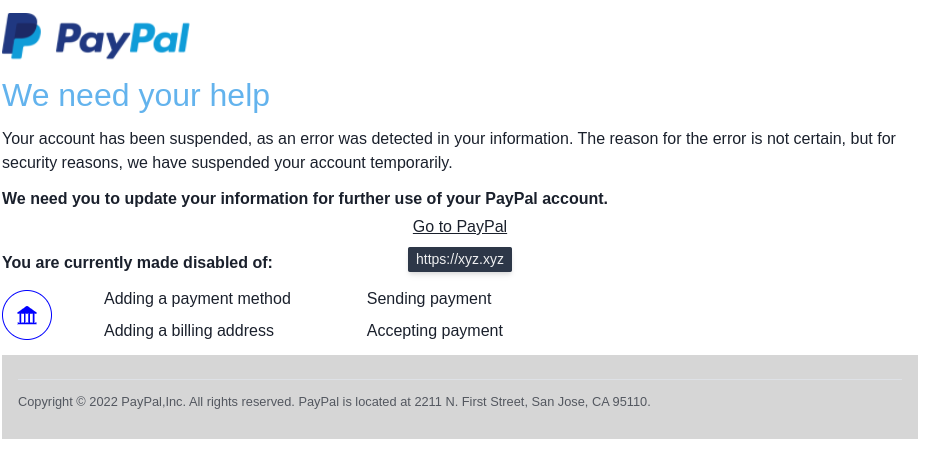
\includegraphics[width=\textwidth]{figures/section2/hide_text.png}

                  \caption{The actual link is hidden behind the text}
                  \label{fig:hide-text}
              }
              \caption{Examples of hiding the actual link behind text or button}
          \end{figure}

          The primary goal of this option is to encourage the user to check for the actual destination links and not to trust the display message.

    \item \textbf{Link shortener}\\
          During our survey of phishing emails, we noticed attackers use URL shorteners to confuse the end-users. A URL shortener is a tool that creates a short, unique URL that will redirect to the specific website of the user choosing. There are multiple free URL shortening services that shorten the URL with a button click. TinyURL, Bitly, Short.io, BL.INK are some popular examples of shortening services. Table \ref{tab:shortener} shows an example of a different URL shortener. The shortened links do not expose the actual domain it redirects to. Phishers use this fact by hiding the actual domain with the help of shortening services.

          \begin{table}[!ht]
              \resizebox{\textwidth}{!}{%
                  \begin{tabular}{l p{0.8\textwidth}}
                      \hline
                      \textbf{Service} & \textbf{Shortener}                                                                              \\
                      \hline
                      Original URL     & https://www.uno.edu/academics/colaehd/ehd/elcf/educational-leadership-graduate-programs/masters \\
                      TinyURL          & https://tinyurl.com/5n6ehd6k                                                                    \\
                      bitly            & https://bit.ly/3CGFfBC                                                                          \\
                      is.gd            & https://is.gd/MKZdLO                                                                            \\
                      Tiny             & http://tiny.cc/unjpuz                                                                           \\
                      RB.GY            & https://rb.gy/nrwbqb                                                                            \\
                      \hline
                  \end{tabular} %
              }

              \caption[URL shortener examples]{Example of different URL shortener and their corresponding shortened links}
              \label{tab:shortener}
          \end{table}

          \begin{figure}[!ht]
              \centering
              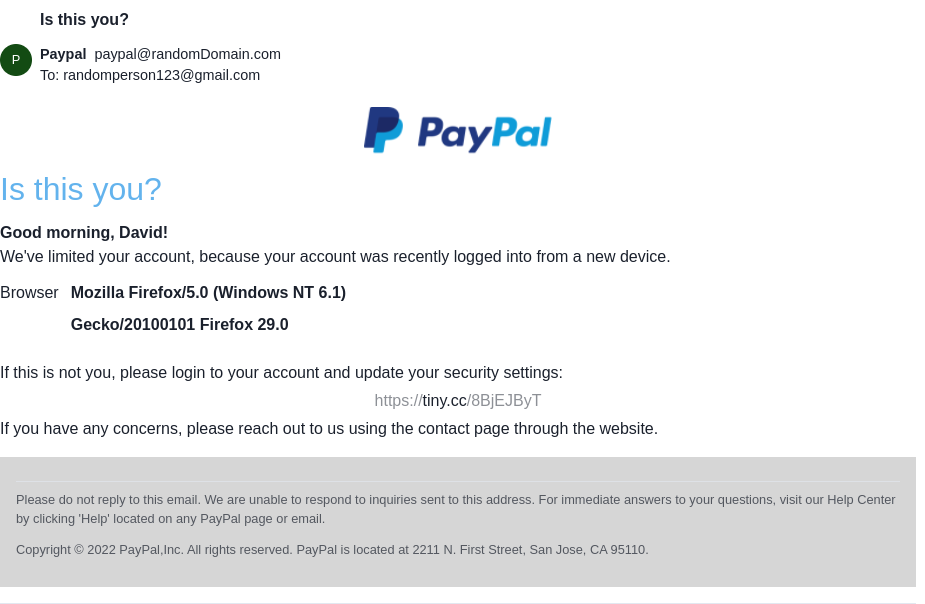
\includegraphics[width=\textwidth]{figures/section2/shortener.png}
              \caption{Example of a URL shortener option in game}
              \label{fig:shortener}
          \end{figure}

          Figure \ref{fig:shortener} shows an example of an email generated with the shortener option. The primary goal of this option is to familiarize players with different URL shortening services and how they can be used to hide actual links. In addition to just knowing how to hide links with shorteners, we want the user to know about different shortening services. Hence, every time the user chooses to hide the link with the shortening service,  we randomly choose one of the shortening services and attach a nano id \footnote{\url{https://github.com/ai/nanoid}} at the end. Table \ref{tab:shortener} shows different link shortener services included in the game with an example.


    \item \textbf{Confusion}\\
          The confusion option teaches users to be careful about familiar links that might look familiar. We focus on subdomains for this option as they are free, can be anything (including existing organization names), and can be added to any existing domains. Phishing links attempt to confuse the users by including the organization name as a subdomain.  We try to show the player this by adding "paypal" to the current domain in the game. For example, "paypal.xyz.xyz" may look like a PayPal domain but is a page in xyz.xyz. Figure \ref{fig:confusion} shows an example of a email generated by the game with link confusion.

          \begin{figure}[!ht]
              \centering
              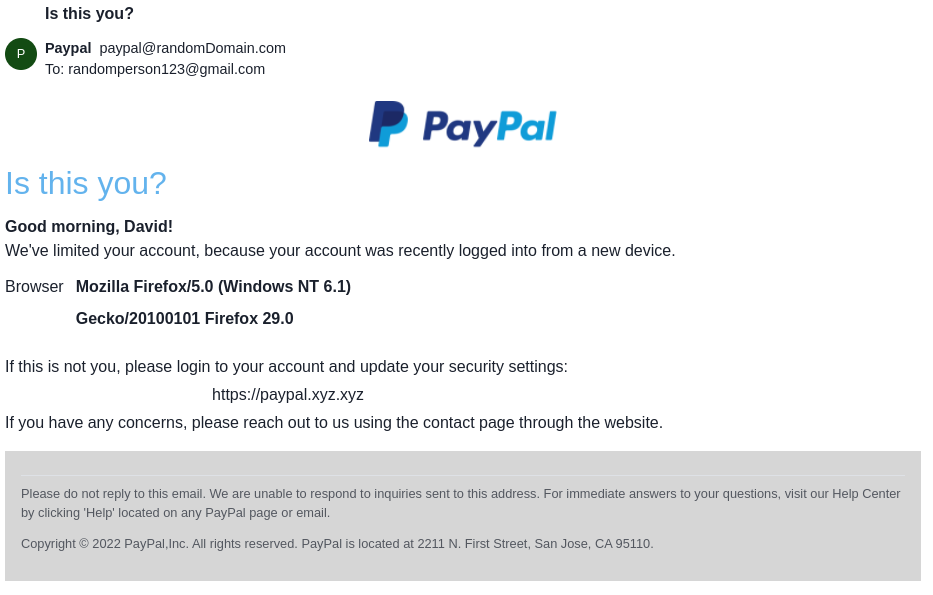
\includegraphics[width=\textwidth]{figures/section2/confusion.png}
              \caption{Example of a email generated with link confusion}
              \label{fig:confusion}
          \end{figure}

    \item \textbf{Display link as is}\\
          The "display link as is" option allows players to see the actual link without modification. This option is useful when the domain purchased by the player is very similar to PayPal. For example, "paypai.com" (with i) looks similar to paypal.com. This domain can easily trick the victims into clicking the link if they are not closely paying attention. We use this option to train users on a similar-looking domain bought from the marketplace.

\end{enumerate}


Player select the link hiding method with an interactive drag and drop approach. We want the player to have immediate feedback on their action. Hence, when the player chooses an option, we immediately change the email. This visualization allows the players to see how the links are used in context to the email.

The final active skill in the game is spoofing. Existing games do not focus on training users on spoofing. However, users can easily get tricked into giving sensitive information if they receive emails from a familiar source. Various free services (Example: figure \ref{fig:spoof_sender}) send emails with custom header (custom to, reply-to, subject fields in the email) without additional verification.

\begin{figure}[!ht]
    \centering
    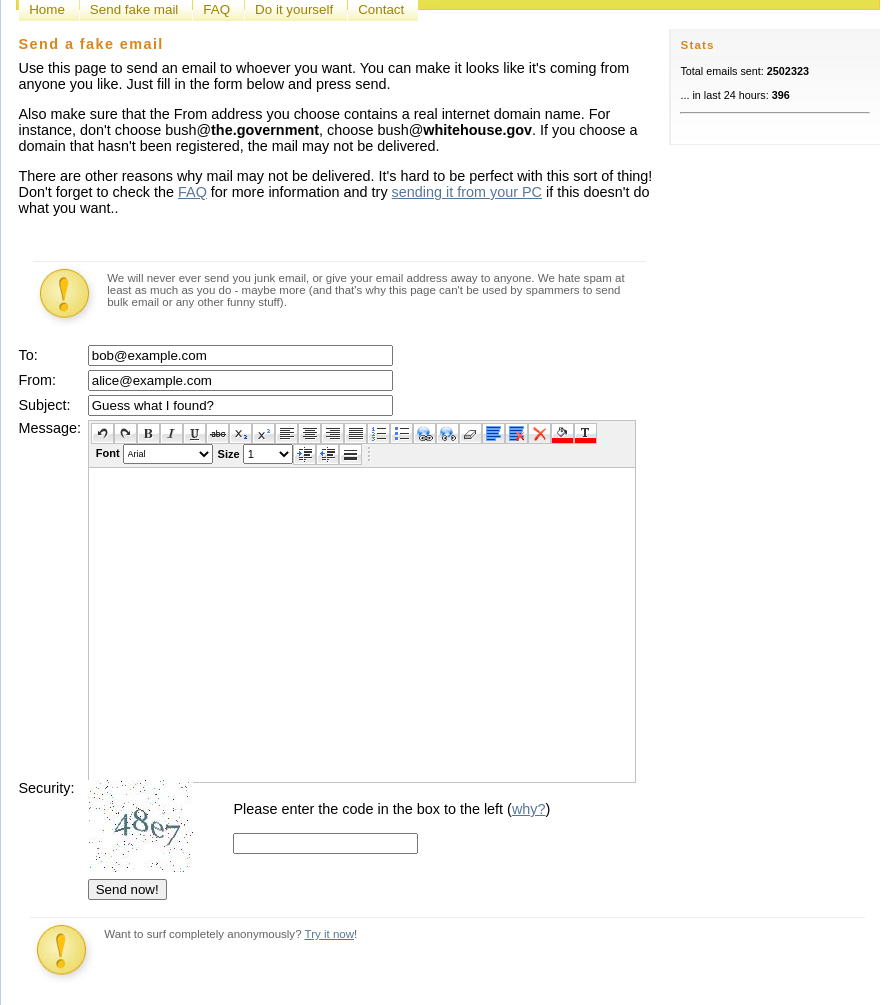
\includegraphics[width=0.9\textwidth]{figures/section2/spoof_sender.png}
    \caption[Fake email sender]{Example of a fake email sender. User can send the email to any email address as any sender.}
    \label{fig:spoof_sender}
\end{figure}

After the player unlocks the "spoof" skill, we allow the player to change the sender's email address to any valid email address. The primary goal is to show the user that the sender can be anyone, and the user has to pay attention to other details of the emails, such as context and links.

\begin{figure}[!ht]
    \centering
    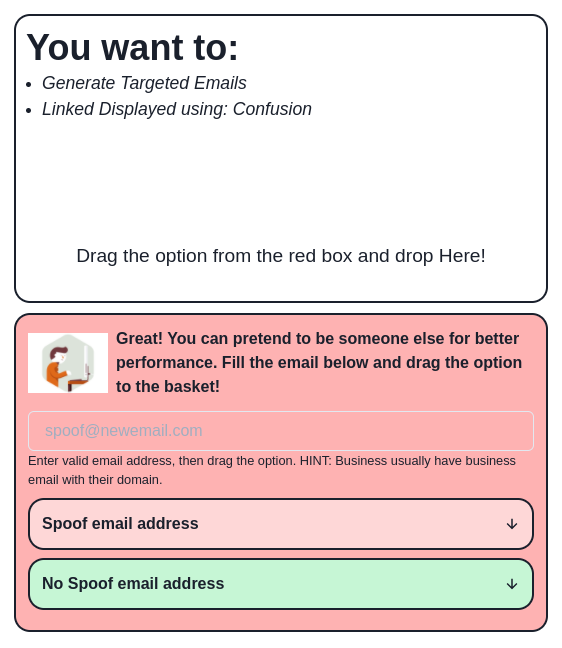
\includegraphics[width=0.4\textwidth]{figures/section2/spoofing.png}
    \caption{Spoofing option in game}
    \label{fig:spoofing}
\end{figure}

\subsection{Email efficiency}
The efficiency of the email generated by the system depends on the options chosen by the user. In our game, higher efficiency correlates to reaching more people and earning more money. Each new skill can improve the efficiency of the email. We calculate the efficiency of generated email as:

\begin{center}
    \resizebox{\textwidth}{!}{
        \begin{math}
            E= \frac{\text{Sum of trained passive skill points + Sum of skill point of active skills chosen by the user}}{\text{Total Available skill points}} \times 100\%
        \end{math}
    }
\end{center}

Table \ref{tab:efficiency} shows the max efficiency point for each skill in the game. The efficiency of passive skills is either 0 (if absent) or max efficiency points (if present), whereas active skills efficiency is calculated based on user input. Active skills options are scaled to show the efficiency of each option. For example, generating targeted (spear phishing) is more efficient as it contains personal information in emails. We add 20 points to the efficiency of the generated email if targeted to replicate this, 0 otherwise.

\begin{table}[!ht]
    \centering
    \begin{tabular}{l c}
        \hline
        Skill                    & Max Efficiency Point \\
        \hline
        Spelling                 & 5                    \\
        Grammar                  & 5                    \\
        Styling                  & 10                   \\
        Research/Targeted Emails & 20                   \\
        Links                    & 25                   \\
        Spoofing                 & 25                   \\
        \hline
    \end{tabular}%
    \caption{Efficiency of each option}
    \label{tab:efficiency}
\end{table}

Different link hiding skills have different efficiency, although close to each other. Hiding the link behind the text gives 18 points, shortening the link gives 20 points, and using confusion gives 25 points. When the player decides to display the link as is, we calculate the string similarity of the user domain with "paypal.com." If the similarity is greater than 80\%, we add 20 points to the efficiency. Else, we add 3 points to efficiency.

Similarly, for spoofing, we want to encourage players to notice that they can pretend to send the email as anyone. We compare the domain (the part after @) in the spoofed email chosen by the user with "paypal.com." We compare the strings as described above with Sørensen-Dice coefficient. Depending on the similarity score, we assign points as shown in table \ref{tab:similarity_spoofed}.

\begin{table}[!ht]
    \centering
    \begin{tabular}{l c}
        \hline
        Similarity & Point \\
        \hline
        90\%       & 20    \\
        80\%       & 18    \\
        60\%       & 7     \\
        Below 60\% & 0     \\
        \hline
    \end{tabular}%
    \caption[Similarity of spoofed email domain and points assigned]{Similarity of spoofed email domain and points assigned. The points are added to active skill points while calculating the efficiency of the email.}
    \label{tab:similarity_spoofed}
\end{table}

We considered different keywords seen in real emails sent by organizations and wanted the players to try these keywords. For example, if the name included keywords "contact," "help," "info," "no-reply," or "noreply," we add 5 points to the efficiency. Similarly, if the email contains "paypal" in the name but was sent from a domain with a low similarity score, we add 10 points.

We calculate the efficiency based on these criteria by adding the player skill points and dividing it by the sum of all available points.

\subsection{Previous Iteration}
The initial version of the game was an open system where users could train with any skill at any given point (given they had enough amount to train) and send as many emails as they wanted. We used time to incentivize users to explore different options and generate efficient emails. The game had the same goals, options, and components but required players to avoid running out of time.

\begin{figure}[!ht]
    \centering
    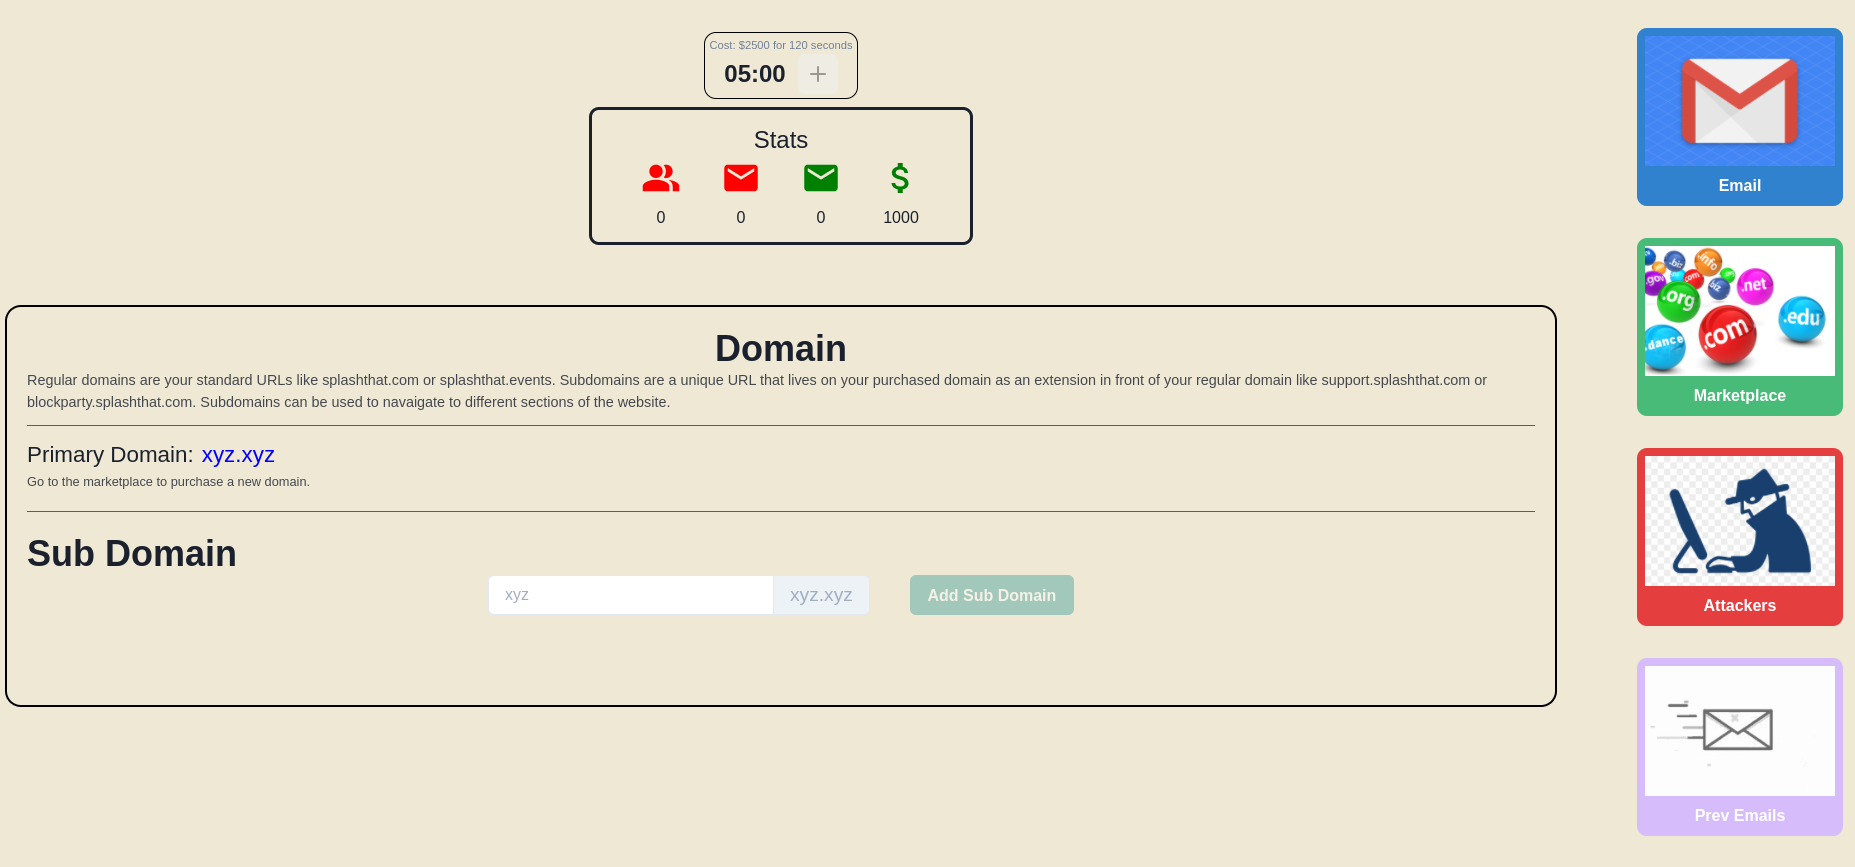
\includegraphics[width=0.9\textwidth]{figures/section2/game_initial.png}
    \caption[Initial version of the game]{Initial version of the game included timer to incentivize the user to complete the game.}
\end{figure}

We noticed a couple of drawbacks during the testing of the initial version. First, we realized that players were constantly worried about running out of time and were not reading the emails and paying attention to all the options. This limitation challenged us to balance the game such that users had enough time to read all the emails but could not brute force (send unlimited emails to achieve the goal) through it. However, different players played the game at different paces, which made us realize that time might not be the best way to incentivize the players to complete the game.

Second, we wanted to ensure that all the players had a similar experience and explored all possible training options. Unfortunately, the open system prevented us from confirming that all the players explored the training module in the same order. It also allowed the player to train on multiple modules simultaneously. Due to this, some combination of training orders allowed players to skip some training modules. For example, players could train spoofing and buy an efficient domain before exploring other training objectives. Since spoofing and good domains are highly efficient, the initial iteration of the game, which allowed players to send unlimited emails, would allow them to complete the game without spending time on other training objectives.

In order to ensure players were exploring all training modules and had the same experience, we developed a new system that lets the player focus on a particular skill at a time. The current design unlocks each skill in part and ensures users are familiar with current techniques before moving on to a new technique.

\subsection{Weekly Goals}
The game's current design divides the game into four parts (weeks). We let the player generate a limited number of emails each week. Each week unlocks new skills the user must train on to achieve the goal (money). Table \ref{tab:weekly-goals} shows skills unlocked each week along with the weekly goals and the number of emails they can send each week. The weekly goals are adjusted based on the maximum possible efficiency of the emails for the current week. As discussed above, the user's current skills determine the efficiency of the email. We played the game multiple times and figured out the best goal to assign for each week. The weekly goals increase each week as we unlock new skills, which leads to more efficient emails.

\begin{table}[ht]
    \centering
    % \resizebox{\textwidth}{!}{%
    \begin{tabular}{c l r r}
        \hline

        \textbf{Week} & \textbf{Trainable Skills}      & \textbf{Weekly Goal} & \textbf{No. of Emails} \\
        \hline
        1             & None                           & 1,500                & 5                      \\
        2             & Spelling, Grammar, Links       & 15,000               & 10                     \\
        3             & Marketplace, Styling, Research & 38,000               & 10                     \\
        4             & Spoofing                       & 80,000               & 10                     \\
        \hline
    \end{tabular}%
    % }
    \caption{Different weeks with their corresponding skills and goals}
    \label{tab:weekly-goals}
\end{table}

Week 1 does not contain any trainable skill and solely focuses on language in the email. We want the player to know that low-tier phishing emails may contain spelling and grammar problems, whereas official/legitimate emails are usually proofread and do not contain these issues.

Week 2 lets the user train on spelling, grammar, and links. Players can remove spelling and grammar errors by training language skills and entirely focus on different link hiding techniques. We let the players play with the link skill by giving a higher number of emails for the week.

Week 3 opens the marketplace along with styling and research. At this point, users have explored different ways to hide the link, and we want to focus on links that might look similar to trick the user. To force users to explore different domains, we disable all link hiding techniques and force users to show the link as is. This forces the player to utilize the marketplace and explore multiple domains.

Finally, week 4 disables the marketplace and unlocks spoofing. We unlock the link hiding skill and let the user play around with all the options. Our initial survey showed players only required half the available emails to figure out spoofing. However, we want the player to play around with all possible combinations for the final few emails, due to which we have a higher number of emails to send than required.
%%%%%%%%%%%%%%%%%%%%%%%%%%%%%%%%%%%%%%%%%%%%%%%%%%%%%%%%%%%%%%%%%%%%%%%
%%%                           System Description
%%%%%%%%%%%%%%%%%%%%%%%%%%%%%%%%%%%%%%%%%%%%%%%%%%%%%%%%%%%%%%%%%%%%%%




\chapter{Evaluation}

The primary goal was to confirm whether our game could improve the correctness of identifying phishing emails with a statistically significant result and understand common patterns found among users who fall for phishing attacks.

\section{Test Design}
Since we want to understand the improvement after the user plays the game, we present each user with pre-survey and post-survey questions. Both surveys contain the same emails, and users have to classify as phishing, legitimate, or need more information (maybe phishing). In addition, we ask the user to provide an optional field to provide feedback on the choice they made.

We curated a list of 12 emails with eight phishing emails and four legitimate emails. We replicated emails from Netflix, a common service used by many individuals. In addition to emails from Netflix, we also had an email from a "co-worker." The context of the email was pre narrated in the survey question. Using emails from a domain different than PayPal allowed us to verify that our game works across multiple domains.

Emails for our evaluation were hand-picked from the most common phishing emails we found during our research (commonly listed in different articles, multiple occurrences in Google searches). The emails include suspicious account warnings such as payment failure, login attempts, suspicious logins, account cancellation, et cetera, and some common too good to be true emails such as free Netflix. We present these emails to the user in a Gmail clone \footnote{\url{https://github.com/codermother/Gmail-Clone}}. Figure \ref{fig:evaluation_site} shows the Gmail clone site with some emails. Although the site looks visually similar to Gmail, it has limited functionality and only allows users to click on "Inbox."

\begin{figure}[!ht]
    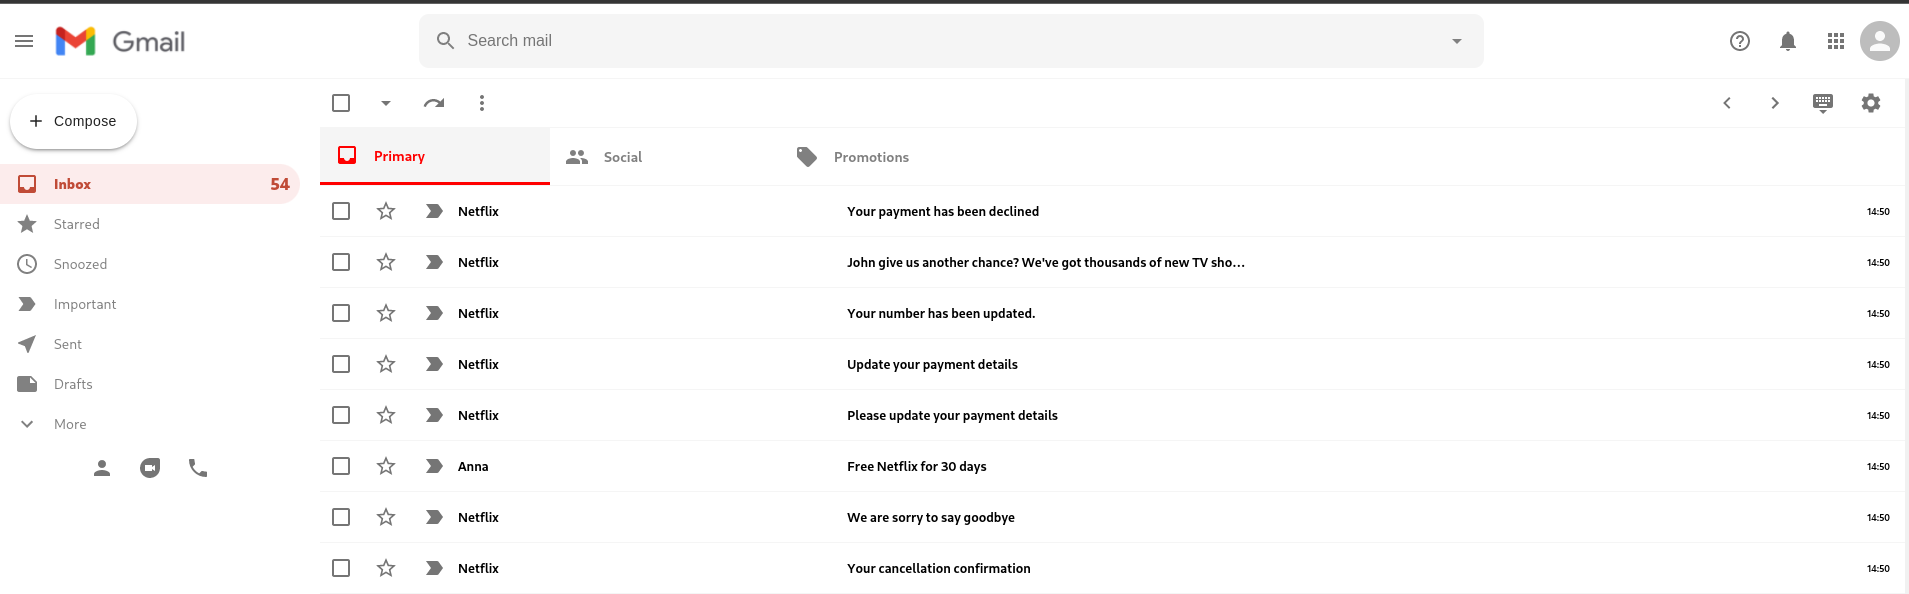
\includegraphics[width=\textwidth]{section3/evaluation_site.png}
    \caption{The Gmail clone used during evaluation with list of custom emails}
    \label{fig:evaluation_site}
\end{figure}

We ask the participants various 5-point Likert scale ratio questions in the post-survey to evaluate engagement. These questions were derived from "Smells Phishy?"\cite{smels_phishy}.

\section{Methodology}
\textbf{Participants}: We distributed the evaluation (along with the game) primarily through email. In addition, we had a group meeting where players completed the survey in person. In total, 13 people attempted the game. However, only 11 participants completed both the presurvey and post-survey. Therefore, we will not consider the data for the two people that did not complete the post-survey. There were four female and seven male participants. All the participants were between 20 and 40, with seven participants in the range 20-30 and 4 participants in the range 30-40. Most of our participants were currently university students, and except for one, all were either enrolled or had a previous background in computer science. The one participant that did not have a Computer Science background had a degree in Biology.

\textbf{Sessions} : All the participants had a single flow for the study.
\begin{enumerate}
    \setlength{\itemsep}{0pt}
    \setlength{\parskip}{0pt}
    \setlength{\topsep}{0pt}
    \item Complete the pre-survey and obtain the passcode for the game. The pre-survey contains some general demographic questions and email classification questions.
    \item  Play the game. We provide the post-survey link after the player completes the game. Players can restart the game from the current week if they fail to complete it in a single try.
    \item Complete the post-survey. The post-survey contains the same set of email classification questions. In addition, it contains questions regarding game engagement.
\end{enumerate}

\textbf{Data Collection}:  We monitor all players' game activities in addition to the data collected through pre-survey and post-survey. This log helps us verify that players played the game in the order we want and can provide hints for future improvements.

\section{Results}
\subsection{Pre-Survey}
The pre-survey responses provided the participant's pre-existing knowledge of phishing scams. Participants chose one of three options (as discussed above in the test design): Phishing, Legitimate, and Need more information (maybe phishing). To understand user thoughts behind their selection, we provide an optional text area to explain their choice.

Each user option is classified as below:

\begin{enumerate}
    \setlength{\itemsep}{0pt}
    \setlength{\parskip}{0pt}
    \setlength{\topsep}{0pt}
    \item \textbf{True Positive}: The user correctly classified the email as phishing.
    \item \textbf{True Negative}: The user correctly classified the email as legitimate.
    \item \textbf{False Positive}: The user incorrectly classified legitimate emails as phishing emails.
    \item \textbf{False Negative}: The user incorrectly classified phishing emails as legitimate emails.
\end{enumerate}

Since participants could mark emails, they are not confident with as "Maybe," we analyze our data in two separate ways, first by neglecting emails marked as "Maybe," and second by including all the results. On average, participants marked 17.41\% of questions as "Maybe" in our presurvey. Since marking an email as "Maybe" shows caution and does not engage the user, we treat these results as "Marked phishing." Hence, phishing emails marked as "Maybe" are classified as "True Positive," and legitimate emails marked as "Maybe" are classified as "False Positive."

Table \ref{tab:pre_survey_responses} shows the average performance (in percent) of each user when we ignore questions marked as "Maybe" and Table \ref{tab:pre_survey_responses_all} show the average perfomance (in percent) when we include all the result and treat "Maybe" as phishing.

\begin{table}[!ht]
    \begin{center}

        \begin{tabular}{c | c c}
            Actual              & \multicolumn{2}{c}{User response}                       \\
                                & \textbf{Phishing}                 & \textbf{Legitimate} \\
            \textbf{Phishing}   & 63\%                              & 37\%                \\
            \textbf{Legitimate} & 7\%                               & 93\%                \\
        \end{tabular}
        \caption[Average performance in pre-survey (I)]{Average performance in pre-survey when we ignore emails marked as "Maybe"}
        \label{tab:pre_survey_responses}
    \end{center}
\end{table}

\begin{table}[!ht]
    \begin{center}

        \begin{tabular}{c | c c}
            Actual              & \multicolumn{2}{c}{User response}                       \\
                                & \textbf{Phishing}                 & \textbf{Legitimate} \\
            \textbf{Phishing}   & 74\%                              & 26\%                \\
            \textbf{Legitimate} & 23\%                              & 77\%                \\
        \end{tabular}
        \caption[Average performance in pre-survey (II)]{Average performance in pre-survey when we include all the results and treat "Maybe" as marked phishing}
        \label{tab:pre_survey_responses_all}
    \end{center}
\end{table}

Participants confidently identified 63\% of phishing emails correctly (when we ignore emails marked as "Maybe"). When we considered emails marked "Maybe," participants detected 74\% phishing emails. Based on these results (See table \ref{tab:pre_survey_responses} and \ref{tab:pre_survey_responses_all}), we can assume participants have some knowledge beforehand about phishing emails. However, we can also see some confusion with some emails based on the number of emails marked as "Maybe" (17.41\%)

We manually reviewed the user text responses to understand why they made each decision. We noticed similar thought processes in many of the participants:

\begin{enumerate}
    \item Participants, who missed phishing emails, were more suspicious of the content of the email and did not focus much on the technical details of the email. For example, some participants thought organizations do not send emails regarding common account information/errors such as subscription cancellation, number update, etc. However, existing popular services commonly send account update emails to the account holder.
    \item Only a couple of participants actively looked at technical details such as the link and the sender. Since participants focused more on the context of the email, any email that asked or put some personal context in the email was marked as potentially phishing or phishing.
\end{enumerate}

\subsection{Game}
Users start the game after the pre-survey. Since we distributed the game through email, we need to verify that the user completed the survey before attempting the game. Therefore, we lock the game with a passcode provided at the end of the pre-survey.

Participants took a little over 25 minutes to complete the game. The fastest recorded time was 18 minutes, and the longest was 43 minutes. We noticed that participants took the longest in Week 3, where they had to play around with different domains. Table \ref{tab:game_time} shows the average time user took for each week.

\begin{table}[!ht]
    \centering
    \begin{tabular}{r r r r }
        \hline
        \textbf{Week} & \textbf{Average Time} & \textbf{Fastest Time} & \textbf{Slowest Time} \\
        1             & 2.27                  & 1.77                  & 2.80                  \\
        2             & 5.18                  & 4.18                  & 6.73                  \\
        3             & 10.54                 & 2.11                  & 18.18                 \\
        4             & 8.54                  & 4.00                  & 23.43                 \\
        \hline
    \end{tabular}
    \caption{Average time user took for each week (in minutes)}
    \label{tab:game_time}
\end{table}

Participants quickly figured out spelling and grammar errors in Week 1 and did not have trouble understanding different link hiding techniques in Week 2. However, many participants had to redo Week 3 as they could not find good domains to try. Some participants tried domains that had no connection with PayPal, such as "starbucks.com," "fredmeyer.com," and "youtube.org." However, participants successfully figured out that purchasing similar domains provided better efficiency. Table \ref{tab:marketplace_domains} shows different domains used in the game.

\begin{table}[!ht]
    \centering
    \begin{tabular}{l c  }
        \hline
        \textbf{Domains}       & \textbf{Number of used} \\
        paypal.org             & 8                       \\
        paypai.com             & 8                       \\
        paypal.co              & 4                       \\
        paypal.nl              & 1                       \\
        info-paypal.com        & 1                       \\
        youtube.org            & 1                       \\
        paypalsupport.com      & 1                       \\
        paypayl-info-gmail.com & 1                       \\
        paypal-paypal.com      & 1                       \\
        billingpal.com         & 1                       \\
        paypay-hotmail.com     & 1                       \\
        paypal.gov             & 1                       \\
        paypal.cm              & 1                       \\
        startbucks.com         & 1                       \\
        fredmeyer.com          & 1                       \\
        \hline
    \end{tabular}
    \caption{Different domains purchased in the marketplace in game}
    \label{tab:marketplace_domains}
\end{table}

Although most participants chose domains with the alternate ending as suggested by the game (when they enter paypal.com), some users were creative and figured our purchasing paypaI.com (with i) would make it look visually similar and be more efficient. We did not consider visual similarity in this iteration, and it can be something to consider in future iterations. Although not visually similar, their

A few participants had a problem with spoofing, but generally, participants quickly understood spoofing and used efficient email addresses. Table \ref{tab:spoofing_emails} shows different emails used by participants during spoofing. Participants used efficient domains (paypal.com) with commonly seen names such as accounts, contact, support, etc.

\begin{table}
    \centering
    \begin{tabular}{l}
        \hline
        \textbf{Emails used by participants} \\
        \hline
        accounts@paypal.com                  \\
        admin@paypal.com                     \\
        alert@paypal.com                     \\
        ben@paypal.com                       \\
        contact@paypal.com                   \\
        customerservice@paypal.com           \\
        paypal@gmail.com                     \\
        paypalsecurity@pp.com                \\
        paypalsupport@paypal.com             \\
        security@paypal.com                  \\
        support@paypal.com                   \\
        \hline
    \end{tabular}
    \caption{Some spoofing emails used by participants}
    \label{tab:spoofing_emails}
\end{table}

Overall, we believe participants were able to play the game smoothly and complete all the game objectives without any hiccups. Furthermore, based on the game logs, players explored all the goals in the game (even though most players had to play the game at least a couple of times).

\subsection{Post-Survey}
The post-survey responses give us an idea of our game's effectiveness by allowing us to compare the before and after game scores. In addition to classifying the emails, we ask the participants 5-point Likert scale questions.

Like pre-evaluation, we evaluate the user performance on two scales, one without emails marked as "Maybe" and one with all the emails. We repeat the same process for the second part (with maybe) as done in the presurvey (Emails marked as "Maybe" are treated as "Phishing").

After playing the game, we noticed participants were more confident in their answers, and on average, participants marked only 10.5\% emails as "Maybe" (7\% improvement from pre-survey).

Table \ref{tab:post_survey_responses} and \ref{tab:post_survey_responses_all} shows participant performance on classifying email after playing the game.


\begin{table}[!ht]
    \begin{center}

        \begin{tabular}{c | c c}
            Actual              & \multicolumn{2}{c}{User response}                       \\
                                & \textbf{Phishing}                 & \textbf{Legitimate} \\
            \textbf{Phishing}   & 80\%                              & 20\%                \\
            \textbf{Legitimate} & 35\%                              & 65\%                \\
        \end{tabular}
        \caption[Average performance in post-survey (I)]{Average performance in post-survey when we do not include emails marked "Maybe"}
        \label{tab:post_survey_responses}
    \end{center}
\end{table}


\begin{table}[!ht]
    \begin{center}

        \begin{tabular}{c | c c}
            Actual              & \multicolumn{2}{c}{User response}                       \\
                                & \textbf{Phishing}                 & \textbf{Legitimate} \\
            \textbf{Phishing}   & 83\%                              & 17\%                \\
            \textbf{Legitimate} & 36\%                              & 64\%                \\
        \end{tabular}
        \caption[Average performance in post-survey (II)]{Average performance in post-survey when we include all the results and treat "Maybe" as marked phishing}
        \label{tab:post_survey_responses_all}
    \end{center}
\end{table}

We manually reviewed user text responses on why they made certain choices (similar to what we did in the pre-survey). We noticed a few common thoughts:

\begin{enumerate}
    \item Participants were paying closer attention to the sender of the emails. However, many participants did not trust emails generated from a subdomain such as mailer.netflix.com. Instead, users believed that companies generally send emails from a primary domain like "netflix.com."
    \item Most of the participants noticed the links hidden under the text. Participants actively avoided links easily detectable as phishing, such as "netflixmovies.com."
    \item Few participants were still untrusting of the content of the email, especially contents with private details such as phone number and credit card info.
\end{enumerate}

\section{Pre vs Post Phishing Knowledge}
Table \ref{tab:pre_vs_post} shows the change in the average score of the participants before and after the game. Although we can not confidently claim that our game improved performance given the sample size and change in score, a few things stand out.

\begin{table}[!ht]
    \centering
    \begin{tabular}{l r r}
        \hline
        \textbf{Answer} & \textbf{A. Change in averge score} & \textbf{B. Change in averge score} \\
        \hline
        True Positive   & 17\%                               & 9\%                                \\
        True Negative   & 2\%                                & -14\%                              \\
        False Positive  & 28\%                               & 14\%                               \\
        False Negative  & -17\%                              & -9\%                               \\
        \hline
    \end{tabular}
    \caption[Change in average score in pre-survey vs post-survey]{Change in average score in pre-survey vs post-survey. Column A. represents change in score when we ignore emails marked as "Maybe" and Column B. represents all the emails when we consider emails marked "Maybe" as phishing.}
    \label{tab:pre_vs_post}
\end{table}

First, participants were more confident in their email classification and marked their email as either phishing or non-phishing. Emails marked as "Maybe" decreased from 17\% to 10\%. For example, one of the participants went from six "Maybe Phishing" to two. Only two out of eleven participants marked more emails as maybe phishing (+1 compared to pre-survey).

Participants were correctly identifying more phishing emails. We see, on average, participants correctly identified 17\% more phishing emails when we ignored emails where participants could not be sure. In addition, participants' performance improved by 9\% even when we treated emails they could not confidently identify as "Phishing."

Our results show that participants were also more skeptical of legitimate emails after playing the game. Participants marked 28\% more legitimate emails as phishing when we don't consider maybe and 14\% more legitimate emails as "Phishing" when we consider all the emails. We saw six participants out of eleven marked at least one of the legitimate emails as phishing.

Overall, we can see that the game positively impacted the participants. Participants were better at identifying phishing emails and all the participants had at least a partial knowledge about protective actions after playing the game. In addition, based on participants' comments, we can see they had at least some knowledge about different objectives of the game.

\subsection{Evaluating emails in post survey}
Out of the eight phishing emails, there were only two emails (Column 1 and Column 5 in figure \ref{fig:emails}) where the user performed significantly worse than other emails. Both the emails had a common theme. All the details looked legitimate, but we hid the actual link under a button. We used "netfiix.com"(with "i"), which is visually similar to "netflix.com," to trick the users.

\begin{figure}[!ht]
    \begin{center}
        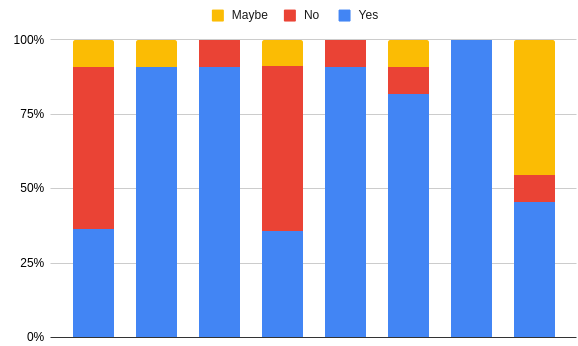
\includegraphics[width=\textwidth]{section3/emails.png}
        \caption{Participants performance on the phishing emails in the evaluation}
        \label{fig:emails}
    \end{center}
\end{figure}

Participants performed well when the sender was not a Netflix domain (netflix.com). Obvious fake domains such as "fakenetflix.com," "netflx.com," "tinyurl.is," and "phishing.com" were caught by the user (Column 6, Column 7, Column 8 in figure \ref{fig:emails}).

\section{Game Time vs perfomance}
We wanted to check if participants spending more time to complete the game performs better. To compare participants' performance before and after the game, we compute the f1-score\footnote{\url{https://en.wikipedia.org/wiki/F-score}} of each participant separately.

\begin{figure}[!ht]
    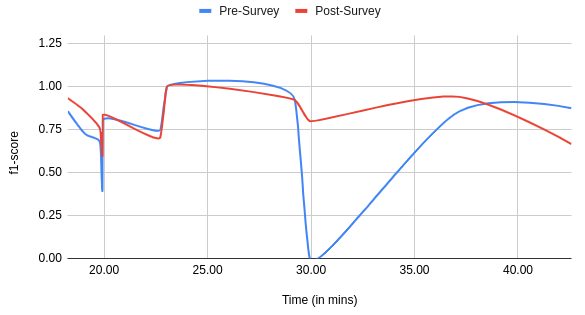
\includegraphics[width=0.9\textwidth]{section3/f1_without.png}
    \caption{Ignoring "Maybe"}
    \label{fig:f1_with_time_a}
\end{figure}

\begin{figure}[!ht]
    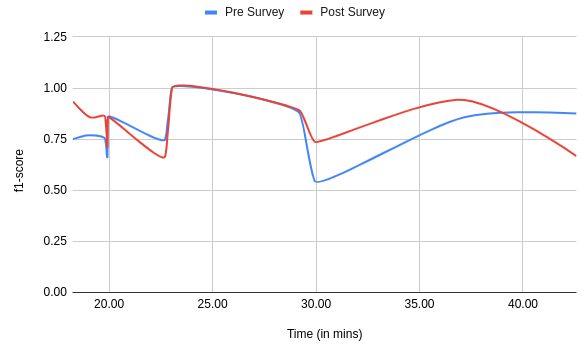
\includegraphics[width=0.9\textwidth]{section3/f1_with.png}
    \caption{Comparison of f1-score before and after playing the game with time (Maybe answers are included)}
    \label{fig:f1_with_time_b}
\end{figure}


Figure \ref{fig:f1_with_time_a} and \ref{fig:f1_with_time_b} show f1-score of each participants with game time. Based on the chart, we can not conclude that higher game time results in better performance. However, we believe that with subtle hints and more emails (that show various passive skills), player playing longer will have better performance.

\section{Questionaire}
Table \ref{tab:game_questions} shows different opinion-based questions asked in the post-survey. The focus of the questionnaire was to assess participants' perceptions and opinions of the game and collect additional feedback about potential improvements.  We used 5-point Likert-scale questions ranging from 1 = strongly disagree to 5 = strongly agree to get feedback.

\begin{table}[!ht]
    \centering
    \begin{tabular}{|r p{0.5\textwidth} r|}
        \hline
            & \textbf{Question}                                                                   & \textbf{Average Rating} \\
        1.  & The game showed phishing tricks.                                                    & 4.90                    \\
        2.  & I better understand phishing scams after playing the game.                          & 4.54                    \\
        3.  & I will use the techniques mentioned in the game to avoid phishing.                  & 3.9                     \\
        4.  & I understand spoofing better.                                                       & 4.18                    \\
        5.  & The game taught me how to protect myself from phishing.                             & 4.27                    \\
        6.  & I learned something new.                                                            & 4.72                    \\
        7.  & I know more about different link hiding techniques and what to look out for.        & 4.27                    \\
        \hline
        8.  & I would like to play the game again.                                                & 2.9                     \\
        9.  & The game is complicated.                                                            & 2.63                    \\
        10. & I prefer reading an educational document to playing a game to learn about phishing. & 1.81                    \\
        11. & Education games are important to understand security.                               & 4.45                    \\
        \hline
    \end{tabular}
    \caption[Likert scale questions relating opinion of the game]{Likert scale questions relating opinion of the game; Higher score means more positive response}
    \label{tab:game_questions}
\end{table}

Questions 1-7 (in table \ref{tab:game_questions}) focus on the educational features of the game and user feelings towards our approach. Based on the average score, we can see that participants welcomed the game and found it helpful. Figure \ref{fig:phishing_game_questions_1} summarizes the distribution of responses for each questions relating to phishing. We had positive responses to the game and the techniques displayed in the game. For example, almost all participants agreed that the game showed phishing tricks, and a majority of participants strongly agreed that the game helped them understand phishing better.

\begin{figure}[!ht]
    \centering
    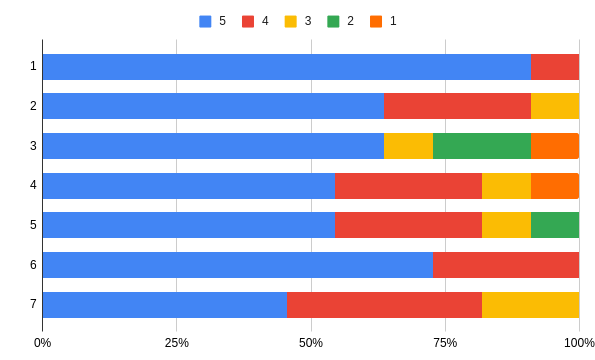
\includegraphics[width=0.8\textwidth]{section3/user_reponse_1.png}
    \caption[Responses to the first 7 questions]{Participants response to the first 7 questions. The numbers correspond to the question numbers in table \ref{tab:game_questions}.}
    \label{fig:phishing_game_questions_1}
\end{figure}

The second set of questions (8-11 in table \ref{tab:game_questions}) is related to participants' general opinions of the game and game-based learning. Figure \ref{fig:phishing_game_questions_2} illustrates the distribution of responses for question through 8-11.  More than half of the participants mentioned that they would not play the game again. We had a chance to talk to many of the participants and got common feedback on the gameplay. They were eager to play it the first time but would not like to play it again.

The majority of the participants did not find the game hard and could complete the game objective. However, we believe the game can be further simplified with better UI and hints to the player.

Finally, we asked participants their opinion on game-based learning. We can see that most of the participants prefer educational games over reading materials. Only one participant favored reading books over educational games for training purposes.


\begin{figure}[!ht]
    \centering
    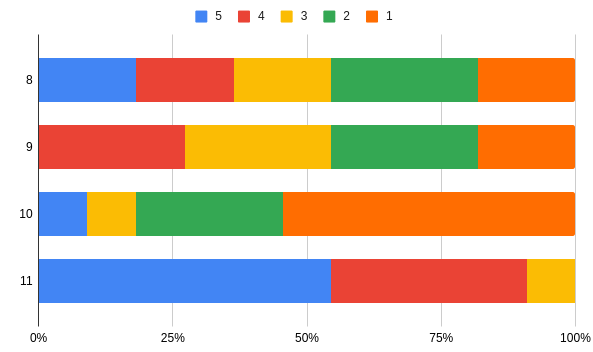
\includegraphics[width=0.8\textwidth]{section3/user_response_2.png}
    \caption[Responses to the 2nd set of questions]{Participants response to questions 8-11. The numbers correspond to the question numbers in table \ref{tab:game_questions}.}
    \label{fig:phishing_game_questions_2}
\end{figure}


\section{Participant Feedback}
At the end of the post-survey, we allow participants to express any comments or improvements to the game. The majority of the comments were positive about the game and pointed out it was a good experience. However, the majority of participants wanted a concise version of the game. One of the participants said he would ask his family to try out the game if it was short.


%%%%%%%%%%%%%%%%%%%%%%%%%%%%%%%%%%%%%%%%%%%%%%%%%%%%%%%%%%%%%%%%%%%%%%%
%%%                           System Description
%%%%%%%%%%%%%%%%%%%%%%%%%%%%%%%%%%%%%%%%%%%%%%%%%%%%%%%%%%%%%%%%%%%%%%




\chapter{Discussion}
- sendInBlue
\section{Limitations}
\section{Future Work}
\section{Conclusion}

%fix spacing in bibliography, if any...
%%%%%%%%%%%%%%%%%%%%%%%%%%%%%%%%%%%%%%%%%%%%%%%%%%%%%%%%%%%%%
\let\oldbibitem\bibitem
\renewcommand{\bibitem}{\setlength{\itemsep}{0pt}\oldbibitem}
%%%%%%%%%%%%%%%%%%%%%%%%%%%%%%%%%%%%%%%%%%%%%%%%%%%%%%%%%%%%%%%
%The bibliography style declared is the IEEE format. If
%you require a different style, see the document
%bibstyles.pdf included in this package. This file,
%hosted by the University of Vienna, shows several
%bibliography styles and examples of in-text citation
%and a references page.
\bibliographystyle{ieeetr}

\phantomsection
\addcontentsline{toc}{chapter}{References}

\renewcommand{\bibname}{{\Large\bf References}}

%This file is a .bib database that contains the sources.
%This removes the dependency on the previous file
%bibliography.tex.
\bibliography{data/myReference}




%This next line includes appendices. The file
%appendix.tex contains commands pointing to
%the appendix files; be sure to change these
%pointers if you end up changing the filenames.
%Leave this commented if you will not need
%appendix material.
% %%%%%%%%%%%%%%%%%%%%%%%%%%%%%%%%%%%%%%%%%%%%%%%%%%%
%
%  New template code for TAMU Theses and Dissertations starting Spring 2021.  
%
%
%  Author: Thesis Office
%  
%  Last Updated: 1/13/2021
%
%%%%%%%%%%%%%%%%%%%%%%%%%%%%%%%%%%%%%%%%%%%%%%%%%%%

\begin{appendices}
\titleformat{\chapter}{\centering\Large}{Appendix \thechapter}{0em}{\vskip .5\baselineskip\centering}
\renewcommand{\appendixname}{Appendix}

%%%%%%%%%%%%%%%%%%%%%%%%%%%%%%%%%%%%%%%%%%%%%%%%%%%%%%%%%%%%%%%%%%%%%%
%%                           APPENDIX A 
%%%%%%%%%%%%%%%%%%%%%%%%%%%%%%%%%%%%%%%%%%%%%%%%%%%%%%%%%%%%%%%%%%%%%

\phantomsection

\chapter{Code snippets}
\label{chap:codesnippets}

\begin{lstlisting}[language=JavaScript, caption=DynamicCompressor fingerprint generation code, label=dynamicCompressorFingerprintGenerationCode]
  getDynamicCompressorFingerprint(): Promise<any>  {
    let sumBuffer = 0;
    let sumBufferHash = null;
    return new Promise((resolve, reject) => {
      try {
        let offlineAudioCtx = new ((<any>window).OfflineAudioContext || (<any>window).webkitOfflineAudioContext)(OFFLINEAUDIOCTX.numberOfChannels, OFFLINEAUDIOCTX.length, OFFLINEAUDIOCTX.sampleRate);
        if (offlineAudioCtx) {
          let oscillator =  offlineAudioCtx.createOscillator();
          oscillator.type = SIGNAL_TYPE;
          oscillator.frequency.value = FREQUENCY;
          
          // Create and configure compressor
          let compressor = offlineAudioCtx.createDynamicsCompressor();
          compressor.threshold && (compressor.threshold.value = COMPRESSOR.threshold);
          compressor.knee && (compressor.knee.value = COMPRESSOR.knee);
          compressor.ratio && (compressor.ratio.value = COMPRESSOR.ratio);
          // compressor.reduction && (compressor.reduction.value = -20);
          compressor.attack && (compressor.attack.value = COMPRESSOR.attack);
          compressor.release && (compressor.release.value = COMPRESSOR.release);

          // Connect nodes
          oscillator.connect(compressor);
          compressor.connect(offlineAudioCtx.destination);

          // Start audio processing
          oscillator.start(0);
          offlineAudioCtx.startRendering();
          offlineAudioCtx.oncomplete = ((evnt: any) => {
            sumBuffer = 0;
            let MD5 =  CryptoJS.algo.MD5.create();
            for (let i = 0; i < evnt.renderedBuffer.length; i++) {
              MD5.update(evnt.renderedBuffer.getChannelData(0)[i].toString());
            }
            const hash = MD5.finalize();
            sumBufferHash = hash.toString(CryptoJS.enc.Hex);
            for (let i = 4500; 5e3 > i; i++) {
              sumBuffer += Math.abs(evnt.renderedBuffer.getChannelData(0)[i]);
            }
            oscillator.disconnect();
            //console.log({"dynamicCompressor": sumBufferHash, "sum": sumBuffer});
            //alert("dynamiccompressor " +sumBufferHash)
            resolve({"hash": sumBufferHash, "sum": sumBuffer, "noFingerprint": false});
          });
        } else {
          reject({"hash": sumBufferHash, "sum": sumBuffer, "noFingerprint": true});
        }
      } catch (u) {
        reject({"hash": sumBufferHash, "sum": sumBuffer, "noFingerprint": true});
      }
    });
  }
\end{lstlisting}

\begin{lstlisting}[language=JavaScript, caption=OscillatorNode fingerprint generation code, label=oscillatorNodeFingerprintGenerationCode]
  getOscillatorNodeFingerprint(): Promise<any>  {
    let oscillatorNode = [];
    let hash = null;
    return new Promise((resolve, reject) => {
      try {
        let audioCtx = new ((<any>window).AudioContext || (<any>window).webkitAudioContext)();
        if (audioCtx) {
          let oscillator = audioCtx.createOscillator();
          let analyser = audioCtx.createAnalyser();
          let gain = audioCtx.createGain();
          let scriptProcessor = audioCtx.createScriptProcessor(SCRIPT_PROCESSOR.bufferSize, SCRIPT_PROCESSOR.numberOfInputChannels, SCRIPT_PROCESSOR.numberOfOutputChannels);
          gain.gain.value = 1; // Disable volume
          analyser.fftSize = 2048;
          oscillator.type = SIGNAL_TYPE // Set oscillator to output wave
          oscillator.connect(analyser); // Connect oscillator output to analyser input
          analyser.connect(scriptProcessor); // Connect analyser output to scriptProcessor input
          scriptProcessor.connect(gain); // Connect scriptProcessor output to gain input
          gain.connect(audioCtx.destination); // Connect gain output to audiocontext destination
          scriptProcessor.onaudioprocess = (async (event) => {
              const bins = new Float32Array(analyser.frequencyBinCount);
              analyser.getFloatFrequencyData(bins);
              for (let i = 0; i < bins.length; i++) {
                oscillatorNode.push(bins[i]);
              }
              analyser.disconnect();
              scriptProcessor.disconnect();
              gain.disconnect();
              const audioFP = JSON.stringify(oscillatorNode);
              hash = CryptoJS.MD5(audioFP).toString();
              await audioCtx.close();
              resolve({"hash": hash, "values": oscillatorNode, "noFingerprint": false});
          });
          oscillator.start(0);
        } else {
          reject({"hash": hash, "values": oscillatorNode, "noFingerprint": true});
        }
      } catch (u) {
        reject({"hash": hash, "values": oscillatorNode, "noFingerprint": true});
      }
    });
  }
\end{lstlisting}

\begin{lstlisting}[language=JavaScript, caption=Hybrid fingerprint generation code, label=hybridFingerprintGenerationCode]
  getHybridFingerprintWithAudioCtx(): Promise<any>  {
    let hybridOscillatorNode = [];
    let hybridHash = null;
    return new Promise((resolve,reject) => {
      try {
        let audioCtx = new ((<any>window).AudioContext || (<any>window).webkitAudioContext)();
        if (audioCtx) {
          let oscillator = audioCtx.createOscillator();
          let analyser = audioCtx.createAnalyser();
          let gain = audioCtx.createGain();
          let scriptProcessor = audioCtx.createScriptProcessor(SCRIPT_PROCESSOR.bufferSize, SCRIPT_PROCESSOR.numberOfInputChannels, SCRIPT_PROCESSOR.numberOfOutputChannels);

          // Create and configure compressor
          let compressor = audioCtx.createDynamicsCompressor();
          compressor.threshold.setValueAtTime(COMPRESSOR.threshold, audioCtx.currentTime);
          compressor.knee.setValueAtTime(COMPRESSOR.knee, audioCtx.currentTime);
          compressor.ratio.setValueAtTime(COMPRESSOR.ratio, audioCtx.currentTime);
          compressor.attack.setValueAtTime(COMPRESSOR.attack, audioCtx.currentTime);
          compressor.release.setValueAtTime(COMPRESSOR.release, audioCtx.currentTime);

          gain.gain.value = 0; // Disable volume
          analyser.fftSize = 2048;
          oscillator.type = SIGNAL_TYPE // Set oscillator to output triangle wave
          oscillator.connect(compressor); // Connect oscillator output to dynamic compressor
          compressor.connect(analyser); // Connect compressor to analyser
          analyser.connect(scriptProcessor); // Connect analyser output to scriptProcessor input
          scriptProcessor.connect(gain); // Connect scriptProcessor output to gain input
          gain.connect(audioCtx.destination); // Connect gain output to audiocontext destination
          scriptProcessor.onaudioprocess = (async (bins: any) => {
              bins = new Float32Array(analyser.frequencyBinCount);
              analyser.getFloatFrequencyData(bins);
              for (let i = 0; i < bins.length; i++) {
                  hybridOscillatorNode.push(bins[i]);
              }
              analyser.disconnect();
              scriptProcessor.disconnect();
              gain.disconnect();
              const audioFP = JSON.stringify(hybridOscillatorNode);
              hybridHash = CryptoJS.MD5(audioFP).toString();
              await audioCtx.close();
              resolve({"hash": hybridHash, "values": hybridOscillatorNode, "noFingerprint": false});
          });
          oscillator.start(0);
        } else {
          reject({"hash": hybridHash, "values": hybridOscillatorNode, "noFingerprint": true});
        }
      } catch (u) {
        reject({"hash": hybridHash, "values": hybridOscillatorNode, "noFingerprint": true});
      }
    });
  }
\end{lstlisting}

\begin{lstlisting}[language=JavaScript, caption=Custom Signal Hybrid fingerprint generation code, label=customSignalHybridFingerprintGenerationCode]
  getCustomSignalHybridFingerprintAudioCtx(): Promise<any>  {
    let hybridOscillatorNode = [];
    let hybridHash = null;
    return new Promise(async (resolve, reject) => {
      try {
        let audioCtx = new ((<any>window).AudioContext || (<any>window).webkitAudioContext)();
        if (audioCtx) {
          const OFFSET = 0.7;
          const pi = Math.PI;
          // https://medium.com/web-audio/phase-offsets-with-web-audio-wavetables-c7dc85ac3218
          // https://meettechniek.info/additional/additive-synthesis.html
          const real = new Float32Array(11);
          const imag = new Float32Array(11);
          real[0] = 0.360;
          real[1] = 0.760;
          real[2] = 0.120;
          real[3] = 0.745;
          real[4] = 0.235;
          real[5] = 0.145;
          real[6] = 0.545;
          real[7] = 0.675;
          real[8] = 0.585;
          real[9] = 0.685;
          real[10] = 0.115;
          real[11] = 0.660;

          imag[0] = pi/2;
          imag[1] = 0;
          imag[2] = pi/2;
          imag[3] = 0;
          imag[4] = pi/2;
          imag[5] = 0;
          imag[6] = pi/2;
          imag[7] = 0;
          imag[8] = pi/2;
          imag[9] = 0;
          imag[10] = pi/2;
          imag[11] = 0

          const wave = audioCtx.createPeriodicWave(real, imag, { disableNormalization: true });
          let oscillator =  audioCtx.createOscillator();
          oscillator.frequency.value = 440;
          oscillator.setPeriodicWave(wave);
          const offset = audioCtx.createConstantSource();
          offset.offset.value = OFFSET;
          let analyser = audioCtx.createAnalyser();
          let gain = audioCtx.createGain();
          let scriptProcessor = audioCtx.createScriptProcessor(SCRIPT_PROCESSOR.bufferSize, SCRIPT_PROCESSOR.numberOfInputChannels, SCRIPT_PROCESSOR.numberOfOutputChannels);

          let compressor = audioCtx.createDynamicsCompressor();
          compressor.threshold.setValueAtTime(COMPRESSOR.threshold, audioCtx.currentTime);
          compressor.knee.setValueAtTime(COMPRESSOR.knee, audioCtx.currentTime);
          compressor.ratio.setValueAtTime(COMPRESSOR.ratio, audioCtx.currentTime);
          compressor.attack.setValueAtTime(COMPRESSOR.attack, audioCtx.currentTime);
          compressor.release.setValueAtTime(COMPRESSOR.release, audioCtx.currentTime);

          gain.gain.value = 0; // Disable volume
          analyser.fftSize = 2048;
          oscillator.connect(compressor); // Connect oscillator output to dynamic compressor
          compressor.connect(analyser); // Connect oscillator output to dynamic compressor
          analyser.connect(scriptProcessor); // Connect analyser output to scriptProcessor input
          scriptProcessor.connect(gain); // Connect scriptProcessor output to gain input
          gain.connect(audioCtx.destination); // Connect gain output to audiocontext destination

          scriptProcessor.onaudioprocess = (async (bins: any) => {
            bins = new Float32Array(analyser.frequencyBinCount);
            analyser.getFloatFrequencyData(bins);
            for (let i = 0; i < bins.length; i++) {
              hybridOscillatorNode.push(bins[i]);
            }
            analyser.disconnect();
            scriptProcessor.disconnect();
            gain.disconnect();
            const audioFP = JSON.stringify(hybridOscillatorNode);
            hybridHash = CryptoJS.MD5(audioFP).toString();
            await audioCtx.close();
            resolve({"hash": hybridHash, "values": hybridOscillatorNode, "noFingerprint": false});
          });
          oscillator.start(0);
          offset.start();
        } else {
          reject({"hash": hybridHash, "values": hybridOscillatorNode, "noFingerprint": true});
        } 
      } catch (u) {
        reject({"hash": hybridHash, "values": hybridOscillatorNode, "noFingerprint": true});
      }
    });
  }
\end{lstlisting}

\begin{lstlisting}[language=JavaScript, caption=Audio Source Hybrid fingerprint generation code, label=audioSourceHybridFingerprintGenerationCode]
  getAudioSourceHybridFingeprintAudioCtx(): Promise<any> {
    let audioData = null;
    let hash= null;
    let analyserNodeData = [];
    return new Promise((resolve, reject) => {
      try {
        const audioContext = new ((<any>window).AudioContext || (<any>window).webkitAudioContext)();
        if (audioContext) {
          const sourceNode = audioContext.createBufferSource();
          const analyserNode = audioContext.createAnalyser();
          const gain = audioContext.createGain();
          const scriptProcessor = audioContext.createScriptProcessor(SCRIPT_PROCESSOR.bufferSize, SCRIPT_PROCESSOR.numberOfInputChannels, SCRIPT_PROCESSOR.numberOfOutputChannels);
           // Create and configure compressor
          const compressor = audioContext.createDynamicsCompressor();
          compressor.threshold.setValueAtTime(COMPRESSOR.threshold, audioContext.currentTime);
          compressor.knee.setValueAtTime(COMPRESSOR.knee, audioContext.currentTime);
          compressor.ratio.setValueAtTime(COMPRESSOR.ratio, audioContext.currentTime);
          compressor.attack.setValueAtTime(COMPRESSOR.attack, audioContext.currentTime);
          compressor.release.setValueAtTime(COMPRESSOR.release, audioContext.currentTime);
          gain.gain.value = 0; // Disable volume
          analyserNode.fftSize = 2048;

          // Now connect the nodes together
          sourceNode.connect(compressor);
          compressor.connect(analyserNode);
          analyserNode.connect(scriptProcessor);
          scriptProcessor.connect(gain);
          gain.connect(audioContext.destination);

          scriptProcessor.onaudioprocess = (async (event: any) => {
            const bins = new Float32Array(analyserNode.frequencyBinCount);
            analyserNode.getFloatFrequencyData(bins);
            for (let i = 0; i < bins.length; i++) {
              analyserNodeData.push(bins[i]);
            }
            const audioFP = JSON.stringify(analyserNodeData);
            hash = CryptoJS.MD5(audioFP).toString();
            gain.disconnect();
            scriptProcessor.disconnect();
            analyserNode.disconnect();
            await audioContext.close();
            resolve({"hash": hash, "values": analyserNodeData, "noFingerprint": false});
          });
          // Load the Audio the first time through, otherwise play it from the buffer
          if(audioData == null) {
            const request = new XMLHttpRequest();
            request.open('GET', '../../../assets/viper-05.ogg', true);
            request.responseType = 'arraybuffer';
            request.onload = (() => {
              audioContext.decodeAudioData(request.response, function(buffer){
                audioData = buffer;
                sourceNode.buffer = buffer;
                sourceNode.start(0);    // Play the sound now
                sourceNode.loop = false;
              },
              function(e){"Error with decoding audio data" + e});
            });
            request.send()
          } else {
            sourceNode.buffer = audioData;
            sourceNode.start(0);    // Play the sound now
            sourceNode.loop = false;
          }
        } else {
          reject({"hash": hash, "values": analyserNodeData, "noFingerprint": true});
        }  
      } catch(u) {
        reject({"hash": hash, "values": analyserNodeData, "noFingerprint": true});
      }  
    });
  }
\end{lstlisting}

\begin{lstlisting}[language=JavaScript, caption=Channel Merge Hybrid fingerprint generation code, label=channelMergeHybridFingerprintGenerationCode]
  getChannelMergeHybridFingerprintAudioCtx(): Promise<any> {
    let hybridHash = null;
    let hybridOscillatorNode = [];
    return new Promise((resolve, reject) => {
      try {
        let audioCtx = new ((<any>window).AudioContext || (<any>window).webkitAudioContext)();
        if (audioCtx) {
          let oscillator1 = audioCtx.createOscillator();
          oscillator1.type = "sine";
          oscillator1.frequency.setValueAtTime(440, audioCtx.currentTime);
          let oscillator2 = audioCtx.createOscillator();
          oscillator2.type = "triangle";
          oscillator2.frequency.setValueAtTime(10000,audioCtx.currentTime);
          let oscillator3 = audioCtx.createOscillator();
          oscillator3.type = "square";
          oscillator3.frequency.setValueAtTime(1880,audioCtx.currentTime);
          let oscillator4 = audioCtx.createOscillator();
          oscillator4.type = "sawtooth";
          oscillator4.frequency.setValueAtTime(22000,audioCtx.currentTime);

          let channelMerger = audioCtx.createChannelMerger(4)
          oscillator1.connect(channelMerger, 0, 0);
          oscillator2.connect(channelMerger, 0, 1);
          oscillator3.connect(channelMerger, 0, 2);
          oscillator4.connect(channelMerger, 0, 3);

          let compressor = audioCtx.createDynamicsCompressor();
          let analyser = audioCtx.createAnalyser();
          let gain = audioCtx.createGain();
          let scriptProcessor = audioCtx.createScriptProcessor(SCRIPT_PROCESSOR.bufferSize, SCRIPT_PROCESSOR.numberOfInputChannels, SCRIPT_PROCESSOR.numberOfOutputChannels);

          compressor.threshold.setValueAtTime(COMPRESSOR.threshold, audioCtx.currentTime);
          compressor.knee.setValueAtTime(COMPRESSOR.knee, audioCtx.currentTime);
          compressor.ratio.setValueAtTime(COMPRESSOR.ratio, audioCtx.currentTime);
          compressor.attack.setValueAtTime(COMPRESSOR.attack, audioCtx.currentTime);
          compressor.release.setValueAtTime(COMPRESSOR.release, audioCtx.currentTime);

          gain.gain.value = 0; // Disable volume
          analyser.fftSize = 4096;
          
          channelMerger.connect(compressor); // Connect merger to compressor
          compressor.connect(analyser); // Connect compressor to analyser
          analyser.connect(scriptProcessor); // Connect analyser output to scriptProcessor input
          scriptProcessor.connect(gain); // Connect scriptProcessor output to gain input
          gain.connect(audioCtx.destination); // Connect gain output to audiocontext destination
    
          scriptProcessor.onaudioprocess = (async (bins: any) => {
              bins = new Float32Array(analyser.frequencyBinCount);
              analyser.getFloatFrequencyData(bins);
              for (let i = 0; i < bins.length; i++) {
                hybridOscillatorNode.push(bins[i]);
              }
              analyser.disconnect();
              scriptProcessor.disconnect();
              gain.disconnect();
              const audioFP = JSON.stringify(hybridOscillatorNode);
              hybridHash = CryptoJS.MD5(audioFP).toString();
              await audioCtx.close();
              resolve({"hash": hybridHash, "values": hybridOscillatorNode, "noFingerprint": false});
          });
          //start source
          oscillator1.start(0);
          oscillator2.start(0);
          oscillator3.start(0);
          oscillator4.start(0);
        } else {
          reject({"hash": hybridHash, "values": hybridOscillatorNode, "noFingerprint": true});
        }
      } catch (u) {
        reject({"hash": hybridHash, "values": hybridOscillatorNode, "noFingerprint": true});
      }
    });
  }
\end{lstlisting}

\begin{lstlisting}[language=JavaScript, caption=Amplitude Modulation Hybrid fingerprint generation code, label=amplitudeModualtionHybridFingerprintGenerationCode]
  getAmplitudeModulationHybridFingerprintAudioCtx(): Promise<any> {
    let hybridOscillatorNode = [];
    let hybridHash = null;
    return new Promise((resolve,reject) => {
      try {
        let audioCtx = new ((<any>window).AudioContext || (<any>window).webkitAudioContext)();
        if (audioCtx) {
          let mod = audioCtx.createOscillator();
          mod.frequency.setValueAtTime(18, audioCtx.currentTime);
          mod.type = "square"
  
          let modGain = audioCtx.createGain();
          modGain.gain.value = 30;
  
          let mod1 = audioCtx.createOscillator();
          mod1.frequency.setValueAtTime(440, audioCtx.currentTime);
          mod1.type = "triangle"
      
          let modGain1 = audioCtx.createGain();
          modGain1.gain.value = 60;
  
          let carrier = audioCtx.createOscillator();
          carrier.type = "sine"
          carrier.frequency.setValueAtTime(10000, audioCtx.currentTime);
          
          let carrierGain = audioCtx.createGain();
          carrierGain.gain.value = 1;

          let analyser = audioCtx.createAnalyser();
          let masterGain = audioCtx.createGain();
          masterGain.gain.value = 0; // Disable volume
          let scriptProcessor = audioCtx.createScriptProcessor(SCRIPT_PROCESSOR.bufferSize, SCRIPT_PROCESSOR.numberOfInputChannels, SCRIPT_PROCESSOR.numberOfOutputChannels);

          mod.connect(modGain);
          mod1.connect(modGain1);
          mod.connect(carrierGain.gain);
          mod1.connect(carrierGain.gain);
          carrier.connect(carrierGain);
          // Create and configure compressor
          let compressor = audioCtx.createDynamicsCompressor();
          compressor.threshold.setValueAtTime(COMPRESSOR.threshold, audioCtx.currentTime);
          compressor.knee.setValueAtTime(COMPRESSOR.knee, audioCtx.currentTime);
          compressor.ratio.setValueAtTime(COMPRESSOR.ratio, audioCtx.currentTime);
          compressor.attack.setValueAtTime(COMPRESSOR.attack, audioCtx.currentTime);
          compressor.release.setValueAtTime(COMPRESSOR.release, audioCtx.currentTime);
          
          analyser.fftSize = 4096;

          carrierGain.connect(compressor); // Connect carrier oscillator output to dynamic compressor
          compressor.connect(analyser); // Connect compressor to analyser
          analyser.connect(scriptProcessor); // Connect analyser output to scriptProcessor input
          scriptProcessor.connect(masterGain); // Connect scriptProcessor output to gain input
          masterGain.connect(audioCtx.destination); // Connect gain output to audiocontext destination
          scriptProcessor.onaudioprocess = (async (bins: any) => {
              bins = new Float32Array(analyser.frequencyBinCount);
              analyser.getFloatFrequencyData(bins);
              for (let i = 0; i < bins.length; i++) {
                  hybridOscillatorNode.push(bins[i]);
              }
              analyser.disconnect();
              scriptProcessor.disconnect();
              masterGain.disconnect();
              const audioFP = JSON.stringify(hybridOscillatorNode);
              hybridHash = CryptoJS.MD5(audioFP).toString();
              await audioCtx.close();
              resolve({"hash": hybridHash, "values": hybridOscillatorNode, "noFingerprint": false});
          });
          carrier.start(0);
          mod.start(0);
          mod1.start(0);
        } else {
          reject({"hash": hybridHash, "values": hybridOscillatorNode, "noFingerprint": true});
        }
      } catch (u) {
        reject({"hash": hybridHash, "values": hybridOscillatorNode, "noFingerprint": true});
      }
    });
  }
\end{lstlisting}

\begin{lstlisting}[language=JavaScript, caption=Frequency Modulation Hybrid  fingerprint generation code, label=frequencyModualtionHybridFingerprintGenerationCode]
  getFrequencyModulationHybridFingerprintAudioCtx(): Promise<any> {
    let hybridOscillatorNode = [];
    let hybridHash = null;
    return new Promise((resolve,reject) => {
      try {
        let audioCtx = new ((<any>window).AudioContext || (<any>window).webkitAudioContext)();
        if (audioCtx) {
          let mod = audioCtx.createOscillator();
          mod.frequency.setValueAtTime(18, audioCtx.currentTime);
          mod.type = "square"
  
          let modGain = audioCtx.createGain();
          modGain.gain.value = 30;
  
          let mod1 = audioCtx.createOscillator();
          mod1.frequency.setValueAtTime(440, audioCtx.currentTime);
          mod1.type = "triangle"
      
          let modGain1 = audioCtx.createGain();
          modGain1.gain.value = 60;
  
          let carrier = audioCtx.createOscillator();
          carrier.type = "sine"
          carrier.frequency.setValueAtTime(10000, audioCtx.currentTime);
          
          let carrierGain = audioCtx.createGain();
          carrierGain.gain.value = 1;

          let analyser = audioCtx.createAnalyser();
          let masterGain = audioCtx.createGain();
          masterGain.gain.value = 0; // Disable volume
          let scriptProcessor = audioCtx.createScriptProcessor(SCRIPT_PROCESSOR.bufferSize, SCRIPT_PROCESSOR.numberOfInputChannels, SCRIPT_PROCESSOR.numberOfOutputChannels);

          mod1.connect(modGain1);
          modGain1.connect(carrier.frequency);
    
          mod.connect(modGain);
          modGain.connect(carrier.frequency);

          // Create and configure compressor
          let compressor = audioCtx.createDynamicsCompressor();
          compressor.threshold.setValueAtTime(COMPRESSOR.threshold, audioCtx.currentTime);
          compressor.knee.setValueAtTime(COMPRESSOR.knee, audioCtx.currentTime);
          compressor.ratio.setValueAtTime(COMPRESSOR.ratio, audioCtx.currentTime);
          compressor.attack.setValueAtTime(COMPRESSOR.attack, audioCtx.currentTime);
          compressor.release.setValueAtTime(COMPRESSOR.release, audioCtx.currentTime);

          carrier.connect(compressor); // Connect carrier output to analyser input
          compressor.connect(analyser); // Connect compressor to analyser
          analyser.connect(scriptProcessor); // Connect analyser output to scriptProcessor input
          scriptProcessor.connect(masterGain); // Connect scriptProcessor output to gain input
          masterGain.connect(audioCtx.destination); // Connect gain output to audiocontext destination
          scriptProcessor.onaudioprocess = (async (bins: any) => {
              bins = new Float32Array(analyser.frequencyBinCount);
              analyser.getFloatFrequencyData(bins);
              for (let i = 0; i < bins.length; i++) {
                  hybridOscillatorNode.push(bins[i]);
              }
              analyser.disconnect();
              scriptProcessor.disconnect();
              masterGain.disconnect();
              const audioFP = JSON.stringify(hybridOscillatorNode);
              hybridHash = CryptoJS.MD5(audioFP).toString();
              await audioCtx.close();
              resolve({"hash": hybridHash, "values": hybridOscillatorNode, "noFingerprint": false});
          });
          carrier.start(0);
          mod.start(0);
          mod1.start(0);
        } else {
          reject({"hash": hybridHash, "values": hybridOscillatorNode, "noFingerprint": true});
        }
      } catch (u) {
        reject({"hash": hybridHash, "values": hybridOscillatorNode, "noFingerprint": true});
      }
    });
  }
\end{lstlisting}



\begin{lstlisting}[language=JavaScript, caption=Expanded Font list, label=expandedfontlist]
["sans-serif-thin","ARNO PRO","Agency FB","Arabic Typesetting","Arial Unicode MS","AvantGarde Bk BT","BankGothic Md BT","Batang","Bitstream Vera Sans Mono","Calibri","Century","Century Gothic","Clarendon","EUROSTILE","Franklin Gothic","Futura Bk BT","Futura Md BT","GOTHAM","Gill Sans","HELV","Haettenschweiler","Helvetica Neue","Humanst521 BT","Leelawadee","Letter Gothic","Levenim MT","Lucida Bright","Lucida Sans","Menlo","MS Mincho","MS Outlook","MS Reference Specialty","MS UI Gothic","MT Extra","MYRIAD PRO","Marlett","Meiryo UI","Microsoft Uighur","Minion Pro","Monotype Corsiva","PMingLiU","Pristina","SCRIPTINA","Segoe UI Light","Serifa","SimHei","Small Fonts","Staccato222 BT","TRAJAN PRO","Univers CE 55 Medium","Vrinda","ZWAdobeF",".Aqua Kana",".Helvetica LT MM",".Times LT MM","18thCentury","8514oem","AR BERKLEY","AR JULIAN","AR PL UKai CN","AR PL UMing CN","AR PL UMing HK","AR PL UMing TW","AR PL UMing TW MBE","Aakar","Abadi MT Condensed Extra Bold","Abadi MT Condensed Light","Abyssinica SIL","AcmeFont","Adobe Arabic","Agency FB","Aharoni","Aharoni Bold","Al Bayan","Al Bayan Bold","Al Bayan Plain","Al Nile","Al Tarikh","Aldhabi","Alfredo","Algerian","Alien Encounters","Almonte Snow","American Typewriter","American Typewriter Bold","American Typewriter Condensed","American Typewriter Light","Amethyst","Andale Mono","Andale Mono Version","Andalus","Angsana New","AngsanaUPC","Ani","AnjaliOldLipi","Aparajita","Apple Braille","Apple Braille Outline 6 Dot","Apple Braille Outline 8 Dot","Apple Braille Pinpoint 6 Dot","Apple Braille Pinpoint 8 Dot","Apple Chancery","Apple Color Emoji","Apple LiGothic Medium","Apple LiSung Light","Apple SD Gothic Neo","Apple SD Gothic Neo Regular","Apple SD GothicNeo ExtraBold","Apple Symbols","AppleGothic","AppleGothic Regular","AppleMyungjo","AppleMyungjo Regular","AquaKana","Arabic Transparent","Arabic Typesetting","Arial","Arial Baltic","Arial Black","Arial Bold","Arial Bold Italic","Arial CE","Arial CYR","Arial Greek","Arial Hebrew","Arial Hebrew Bold","Arial Italic","Arial Narrow","Arial Narrow Bold","Arial Narrow Bold Italic","Arial Narrow Italic","Arial Rounded Bold","Arial Rounded MT Bold","Arial TUR","Arial Unicode MS","ArialHB","Arimo","Asimov","Autumn","Avenir","Avenir Black","Avenir Book","Avenir Next","Avenir Next Bold","Avenir Next Condensed","Avenir Next Condensed Bold","Avenir Next Demi Bold","Avenir Next Heavy","Avenir Next Regular","Avenir Roman","Ayuthaya","BN Jinx","BN Machine","BOUTON International Symbols","BabyKruffy","Baghdad","Bahnschrift","Balthazar","Bangla MN","Bangla MN Bold","Bangla Sangam MN","Bangla Sangam MN Bold","Baskerville","Baskerville Bold","Baskerville Bold Italic","Baskerville Old Face","Baskerville SemiBold","Baskerville SemiBold Italic","Bastion","Batang","BatangChe","Bauhaus 93","Beirut","Bell MT","Bell MT Bold","Bell MT Italic","Bellerose","Berlin Sans FB","Berlin Sans FB Demi","Bernard MT Condensed","BiauKai","Big Caslon","Big Caslon Medium","Birch Std","Bitstream Charter","Bitstream Vera Sans","Blackadder ITC","Blackoak Std","Bobcat","Bodoni 72","Bodoni MT","Bodoni MT Black","Bodoni MT Poster Compressed","Bodoni Ornaments","BolsterBold","Book Antiqua","Book Antiqua Bold","Bookman Old Style","Bookman Old Style Bold","Bookshelf Symbol 7","Borealis","Bradley Hand","Bradley Hand ITC","Braggadocio","Brandish","Britannic Bold","Broadway","Browallia New","BrowalliaUPC","Brush Script","Brush Script MT","Brush Script MT Italic","Brush Script Std","Brussels","Calibri","Calibri Bold","Calibri Light","Californian FB","Calisto MT","Calisto MT Bold","Calligraphic","Calvin","Cambria","Cambria Bold","Cambria Math","Candara","Candara Bold","Candles","Carrois Gothic SC","Castellar","Centaur","Century","Century Gothic","Century Gothic Bold","Century Schoolbook","Century Schoolbook Bold","Century Schoolbook L","Chalkboard","Chalkboard Bold","Chalkboard SE","Chalkboard SE Bold","ChalkboardBold","Chalkduster","Chandas","Chaparral Pro","Chaparral Pro Light","Charlemagne Std","Charter","Chilanka","Chiller","Chinyen","Clarendon","Cochin","Cochin Bold","Colbert","Colonna MT","Comic Sans MS","Comic Sans MS Bold","Commons","Consolas","Consolas Bold","Constantia","Constantia Bold","Coolsville","Cooper Black","Cooper Std Black","Copperplate","Copperplate Bold","Copperplate Gothic Bold","Copperplate Light","Corbel","Corbel Bold","Cordia New","CordiaUPC","Corporate","Corsiva","Corsiva Hebrew","Corsiva Hebrew Bold","Courier","Courier 10 Pitch","Courier Bold","Courier New","Courier New Baltic","Courier New Bold","Courier New CE","Courier New Italic","Courier Oblique","Cracked Johnnie","Creepygirl","Curlz MT","Cursor","Cutive Mono","DFKai-SB","DIN Alternate","DIN Condensed","Damascus","Damascus Bold","Dancing Script","DaunPenh","David","Dayton","DecoType Naskh","Deja Vu","DejaVu LGC Sans","DejaVu Sans","DejaVu Sans Mono","DejaVu Serif","Deneane","Desdemona","Detente","Devanagari MT","Devanagari MT Bold","Devanagari Sangam MN","Didot","Didot Bold","Digifit","DilleniaUPC","Dingbats","Distant Galaxy","Diwan Kufi","Diwan Kufi Regular","Diwan Thuluth","Diwan Thuluth Regular","DokChampa","Dominican","Dotum","DotumChe","Droid Sans","Droid Sans Fallback","Droid Sans Mono","Dyuthi","Ebrima","Edwardian Script ITC","Elephant","Emmett","Engravers MT","Engravers MT Bold","Enliven","Eras Bold ITC","Estrangelo Edessa","Ethnocentric","EucrosiaUPC","Euphemia","Euphemia UCAS","Euphemia UCAS Bold","Eurostile","Eurostile Bold","Expressway Rg","FangSong","Farah","Farisi","Felix Titling","Fingerpop","Fixedsys","Flubber","Footlight MT Light","Forte","FrankRuehl","Frankfurter Venetian TT","Franklin Gothic Book","Franklin Gothic Book Italic","Franklin Gothic Medium","Franklin Gothic Medium Cond","Franklin Gothic Medium Italic","FreeMono","FreeSans","FreeSerif","FreesiaUPC","Freestyle Script","French Script MT","Futura","Futura Condensed ExtraBold","Futura Medium","GB18030 Bitmap","Gabriola","Gadugi","Garamond","Garamond Bold","Gargi","Garuda","Gautami","Gazzarelli","Geeza Pro","Geeza Pro Bold","Geneva","GenevaCY","Gentium","Gentium Basic","Gentium Book Basic","GentiumAlt","Georgia","Georgia Bold","Geotype TT","Giddyup Std","Gigi","Gill","Gill Sans","Gill Sans Bold","Gill Sans MT","Gill Sans MT Bold","Gill Sans MT Condensed","Gill Sans MT Ext Condensed Bold","Gill Sans MT Italic","Gill Sans Ultra Bold","Gill Sans Ultra Bold Condensed","Gisha","Glockenspiel","Gloucester MT Extra Condensed","Good Times","Goudy","Goudy Old Style","Goudy Old Style Bold","Goudy Stout","Greek Diner Inline TT","Gubbi","Gujarati MT","Gujarati MT Bold","Gujarati Sangam MN","Gujarati Sangam MN Bold","Gulim","GulimChe","GungSeo Regular","Gungseouche","Gungsuh","GungsuhChe","Gurmukhi","Gurmukhi MN","Gurmukhi MN Bold","Gurmukhi MT","Gurmukhi Sangam MN","Gurmukhi Sangam MN Bold","Haettenschweiler","Hand Me Down S (BRK)","Hansen","Harlow Solid Italic","Harrington","Harvest","HarvestItal","Haxton Logos TT","HeadLineA Regular","HeadlineA","Heavy Heap","Hei","Hei Regular","Heiti SC","Heiti SC Light","Heiti SC Medium","Heiti TC","Heiti TC Light","Heiti TC Medium","Helvetica","Helvetica Bold","Helvetica CY Bold","Helvetica CY Plain","Helvetica LT Std","Helvetica Light","Helvetica Neue","Helvetica Neue Bold","Helvetica Neue Medium","Helvetica Oblique","HelveticaCY","HelveticaNeueLT Com 107 XBlkCn","Herculanum","High Tower Text","Highboot","Hiragino Kaku Gothic Pro W3","Hiragino Kaku Gothic Pro W6","Hiragino Kaku Gothic ProN W3","Hiragino Kaku Gothic ProN W6","Hiragino Kaku Gothic Std W8","Hiragino Kaku Gothic StdN W8","Hiragino Maru Gothic Pro W4","Hiragino Maru Gothic ProN W4","Hiragino Mincho Pro W3","Hiragino Mincho Pro W6","Hiragino Mincho ProN W3","Hiragino Mincho ProN W6","Hiragino Sans GB W3","Hiragino Sans GB W6","Hiragino Sans W0","Hiragino Sans W1","Hiragino Sans W2","Hiragino Sans W3","Hiragino Sans W4","Hiragino Sans W5","Hiragino Sans W6","Hiragino Sans W7","Hiragino Sans W8","Hiragino Sans W9","Hobo Std","Hoefler Text","Hoefler Text Black","Hoefler Text Ornaments","Hollywood Hills","Hombre","Huxley Titling","ITC Stone Serif","ITF Devanagari","ITF Devanagari Marathi","ITF Devanagari Medium","Impact","Imprint MT Shadow","InaiMathi","Induction","Informal Roman","Ink Free","IrisUPC","Iskoola Pota","Italianate","Jamrul","JasmineUPC","JavaneseText","Jokerman","JuiceITC","KacstArt","KacstBook","KacstDecorative","KacstDigital","KacstFarsi","KacstLetter","KacstNaskh","KacstOffice","KacstOne","KacstPen","KacstPoster","KacstQurn","KacstScreen","KacstTitle","KacstTitleL","Kai","Kai Regular","KaiTi","Kailasa","Kailasa Regular","Kaiti SC","Kaiti SC Black","Kalapi","Kalimati","Kalinga","Kannada MN","Kannada MN Bold","Kannada Sangam MN","Kannada Sangam MN Bold","Kartika","Karumbi","Kedage","Kefa","Kefa Bold","Keraleeyam","Keyboard","Khmer MN","Khmer MN Bold","Khmer OS","Khmer OS System","Khmer Sangam MN","Khmer UI","Kinnari","Kino MT","KodchiangUPC","Kohinoor Bangla","Kohinoor Devanagari","Kohinoor Telugu","Kokila","Kokonor","Kokonor Regular","Kozuka Gothic Pr6N B","Kristen ITC","Krungthep","KufiStandardGK","KufiStandardGK Regular","Kunstler Script","Laksaman","Lao MN","Lao Sangam MN","Lao UI","LastResort","Latha","Leelawadee","Letter Gothic Std","LetterOMatic!","Levenim MT","LiHei Pro","LiSong Pro","Liberation Mono","Liberation Sans","Liberation Sans Narrow","Liberation Serif","Likhan","LilyUPC","Limousine","Lithos Pro Regular","LittleLordFontleroy","Lohit Assamese","Lohit Bengali","Lohit Devanagari","Lohit Gujarati","Lohit Gurmukhi","Lohit Hindi","Lohit Kannada","Lohit Malayalam","Lohit Odia","Lohit Punjabi","Lohit Tamil","Lohit Tamil Classical","Lohit Telugu","Loma","Lucida Blackletter","Lucida Bright","Lucida Bright Demibold","Lucida Bright Demibold Italic","Lucida Bright Italic","Lucida Calligraphy","Lucida Calligraphy Italic","Lucida Console","Lucida Fax","Lucida Fax Demibold","Lucida Fax Regular","Lucida Grande","Lucida Grande Bold","Lucida Handwriting","Lucida Handwriting Italic","Lucida Sans","Lucida Sans Demibold Italic","Lucida Sans Typewriter","Lucida Sans Typewriter Bold","Lucida Sans Unicode","Luminari","Luxi Mono","MS Gothic","MS Mincho","MS Outlook","MS PGothic","MS PMincho","MS Reference Sans Serif","MS Reference Specialty","MS Sans Serif","MS Serif","MS UI Gothic","MT Extra","MV Boli","Mael","Magneto","Maiandra GD","Malayalam MN","Malayalam MN Bold","Malayalam Sangam MN","Malayalam Sangam MN Bold","Malgun Gothic","Mallige","Mangal","Manorly","Marion","Marion Bold","Marker Felt","Marker Felt Thin","Marlett","Martina","Matura MT Script Capitals","Meera","Meiryo","Meiryo Bold","Meiryo UI","MelodBold","Menlo","Menlo Bold","Mesquite Std","Microsoft","Microsoft Himalaya","Microsoft JhengHei","Microsoft JhengHei UI","Microsoft New Tai Lue","Microsoft PhagsPa","Microsoft Sans Serif","Microsoft Tai Le","Microsoft Tai Le Bold","Microsoft Uighur","Microsoft YaHei","Microsoft YaHei UI","Microsoft Yi Baiti","Minerva","MingLiU","MingLiU-ExtB","MingLiU_HKSCS","Minion Pro","Miriam","Mishafi","Mishafi Gold","Mistral","Modern","Modern No. 20","Monaco","Mongolian Baiti","Monospace","Monotype Corsiva","Monotype Sorts","MoolBoran","Moonbeam","MotoyaLMaru","Mshtakan","Mshtakan Bold","Mukti Narrow","Muna","Myanmar MN","Myanmar MN Bold","Myanmar Sangam MN","Myanmar Text","Mycalc","Myriad Arabic","Myriad Hebrew","Myriad Pro","NISC18030","NSimSun","Nadeem","Nadeem Regular","Nakula","Nanum Barun Gothic","Nanum Gothic","Nanum Myeongjo","NanumBarunGothic","NanumGothic","NanumGothic Bold","NanumGothicCoding","NanumMyeongjo","NanumMyeongjo Bold","Narkisim","Nasalization","Navilu","Neon Lights","New Peninim MT","New Peninim MT Bold","News Gothic MT","News Gothic MT Bold","Niagara Engraved","Niagara Solid","Nimbus Mono L","Nimbus Roman No9 L","Nimbus Sans L","Nimbus Sans L Condensed","Nina","Nirmala UI","Nirmala.ttf","Norasi","Noteworthy","Noteworthy Bold","Noto Color Emoji","Noto Emoji","Noto Mono","Noto Naskh Arabic","Noto Nastaliq Urdu","Noto Sans","Noto Sans Armenian","Noto Sans Bengali","Noto Sans CJK","Noto Sans Canadian Aboriginal","Noto Sans Cherokee","Noto Sans Devanagari","Noto Sans Ethiopic","Noto Sans Georgian","Noto Sans Gujarati","Noto Sans Gurmukhi","Noto Sans Hebrew","Noto Sans JP","Noto Sans KR","Noto Sans Kannada","Noto Sans Khmer","Noto Sans Lao","Noto Sans Malayalam","Noto Sans Myanmar","Noto Sans Oriya","Noto Sans SC","Noto Sans Sinhala","Noto Sans Symbols","Noto Sans TC","Noto Sans Tamil","Noto Sans Telugu","Noto Sans Thai","Noto Sans Yi","Noto Serif","Notram","November","Nueva Std","Nueva Std Cond","Nyala","OCR A Extended","OCR A Std","Old English Text MT","OldeEnglish","Onyx","OpenSymbol","OpineHeavy","Optima","Optima Bold","Optima Regular","Orator Std","Oriya MN","Oriya MN Bold","Oriya Sangam MN","Oriya Sangam MN Bold","Osaka","Osaka-Mono","OsakaMono","PCMyungjo Regular","PCmyoungjo","PMingLiU","PMingLiU-ExtB","PR Celtic Narrow","PT Mono","PT Sans","PT Sans Bold","PT Sans Caption Bold","PT Sans Narrow Bold","PT Serif","Padauk","Padauk Book","Padmaa","Pagul","Palace Script MT","Palatino","Palatino Bold","Palatino Linotype","Palatino Linotype Bold","Papyrus","Papyrus Condensed","Parchment","Parry Hotter","PenultimateLight","Perpetua","Perpetua Bold","Perpetua Titling MT","Perpetua Titling MT Bold","Phetsarath OT","Phosphate","Phosphate Inline","Phosphate Solid","PhrasticMedium","PilGi Regular","Pilgiche","PingFang HK","PingFang SC","PingFang TC","Pirate","Plantagenet Cherokee","Playbill","Poor Richard","Poplar Std","Pothana2000","Prestige Elite Std","Pristina","Purisa","QuiverItal","Raanana","Raanana Bold","Raavi","Rachana","Rage Italic","RaghuMalayalam","Ravie","Rekha","Roboto","Rockwell","Rockwell Bold","Rockwell Condensed","Rockwell Extra Bold","Rockwell Italic","Rod","Roland","Rondalo","Rosewood Std Regular","RowdyHeavy","Russel Write TT","SF Movie Poster","STFangsong","STHeiti","STIXGeneral","STIXGeneral-Bold","STIXGeneral-Regular","STIXIntegralsD","STIXIntegralsD-Bold","STIXIntegralsSm","STIXIntegralsSm-Bold","STIXIntegralsUp","STIXIntegralsUp-Bold","STIXIntegralsUp-Regular","STIXIntegralsUpD","STIXIntegralsUpD-Bold","STIXIntegralsUpD-Regular","STIXIntegralsUpSm","STIXIntegralsUpSm-Bold","STIXNonUnicode","STIXNonUnicode-Bold","STIXSizeFiveSym","STIXSizeFiveSym-Regular","STIXSizeFourSym","STIXSizeFourSym-Bold","STIXSizeOneSym","STIXSizeOneSym-Bold","STIXSizeThreeSym","STIXSizeThreeSym-Bold","STIXSizeTwoSym","STIXSizeTwoSym-Bold","STIXVariants","STIXVariants-Bold","STKaiti","STSong","STXihei","SWGamekeys MT","Saab","Sahadeva","Sakkal Majalla","Salina","Samanata","Samyak Devanagari","Samyak Gujarati","Samyak Malayalam","Samyak Tamil","Sana","Sana Regular","Sans","Sarai","Sathu","Savoye LET Plain:1.0","Sawasdee","Script","Script MT Bold","Segoe MDL2 Assets","Segoe Print","Segoe Pseudo","Segoe Script","Segoe UI","Segoe UI Emoji","Segoe UI Historic","Segoe UI Semilight","Segoe UI Symbol","Serif","Shonar Bangla","Showcard Gothic","Shree Devanagari 714","Shruti","SignPainter-HouseScript","Silom","SimHei","SimSun","SimSun-ExtB","Simplified Arabic","Simplified Arabic Fixed","Sinhala MN","Sinhala MN Bold","Sinhala Sangam MN","Sinhala Sangam MN Bold","Sitka","Skia","Skia Regular","Skinny","Small Fonts","Snap ITC","Snell Roundhand","Snowdrift","Songti SC","Songti SC Black","Songti TC","Source Code Pro","Splash","Standard Symbols L","Stencil","Stencil Std","Stephen","Sukhumvit Set","Suruma","Sylfaen","Symbol","Symbole","System","System Font","TAMu_Kadambri","TAMu_Kalyani","TAMu_Maduram","TSCu_Comic","TSCu_Paranar","TSCu_Times","Tahoma","Tahoma Negreta","TakaoExGothic","TakaoExMincho","TakaoGothic","TakaoMincho","TakaoPGothic","TakaoPMincho","Tamil MN","Tamil MN Bold","Tamil Sangam MN","Tamil Sangam MN Bold","Tarzan","Tekton Pro","Tekton Pro Cond","Tekton Pro Ext","Telugu MN","Telugu MN Bold","Telugu Sangam MN","Telugu Sangam MN Bold","Tempus Sans ITC","Terminal","Terminator Two","Thonburi","Thonburi Bold","Tibetan Machine Uni","Times","Times Bold","Times New Roman","Times New Roman Baltic","Times New Roman Bold","Times New Roman Italic","Times Roman","Tlwg Mono","Tlwg Typewriter","Tlwg Typist","Tlwg Typo","TlwgMono","TlwgTypewriter","Toledo","Traditional Arabic","Trajan Pro","Trattatello","Trebuchet MS","Trebuchet MS Bold","Tunga","Tw Cen MT","Tw Cen MT Bold","Tw Cen MT Italic","URW Bookman L","URW Chancery L","URW Gothic L","URW Palladio L","Ubuntu","Ubuntu Condensed","Ubuntu Mono","Ukai","Ume Gothic","Ume Mincho","Ume P Gothic","Ume P Mincho","Ume UI Gothic","Uming","Umpush","UnBatang","UnDinaru","UnDotum","UnGraphic","UnGungseo","UnPilgi","Untitled1","Urdu Typesetting","Uroob","Utkal","Utopia","Utsaah","Valken","Vani","Vemana2000","Verdana","Verdana Bold","Vijaya","Viner Hand ITC","Vivaldi","Vivian","Vladimir Script","Vrinda","Waree","Waseem","Waverly","Webdings","WenQuanYi Bitmap Song","WenQuanYi Micro Hei","WenQuanYi Micro Hei Mono","WenQuanYi Zen Hei","Whimsy TT","Wide Latin","Wingdings","Wingdings 2","Wingdings 3","Woodcut","X-Files","Year supply of fairy cakes","Yu Gothic","Yu Mincho","Yuppy SC","Yuppy SC Regular","Yuppy TC","Yuppy TC Regular","Zapf Dingbats","Zapfino","Zawgyi-One","gargi","lklug","mry_KacstQurn","ori1Uni"]
\end{lstlisting}
%%%%%%%%%%%%%%%%%%%%%%%%%%%%%%%%%%%%%%%%%%%%%%%%%%%%%%%%%%%%%%%%%%%%%%
%%                           APPENDIX B
%%%%%%%%%%%%%%%%%%%%%%%%%%%%%%%%%%%%%%%%%%%%%%%%%%%%%%%%%%%%%%%%%%%%%

\chapter{Figures}
\begin{figure}[H]
    \centering
    \subfloat[\centering Dynamic Compressor]{{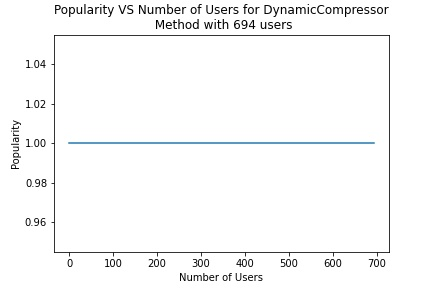
\includegraphics[scale=0.5]{CDF/DynamicCompressor_CDF.jpeg}}}%
    \qquad
    \subfloat[\centering Oscillator Node]{{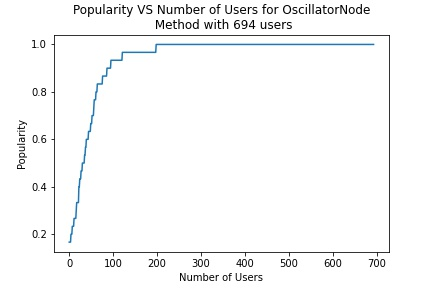
\includegraphics[scale=0.5]{CDF/OscillatorNode_CDF.jpeg}}}%
    \qquad
    \subfloat[\centering Hybrid]{{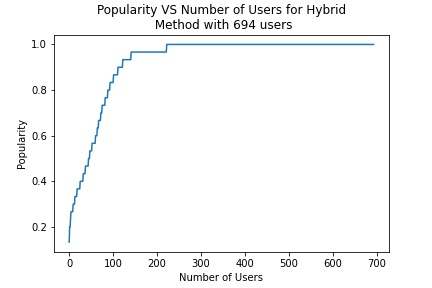
\includegraphics[scale=0.5]{CDF/Hybrid_CDF.jpeg}}}%
    \qquad
    \subfloat[\centering Custom Signal Hybrid]{{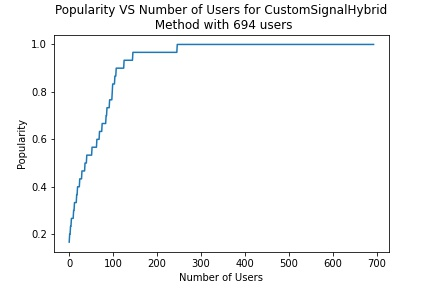
\includegraphics[scale=0.5]{CDF/CustomSignalHybrid_CDF.jpeg}}}%
    \qquad
    \caption[{The frequency of the highest occurring fingerprint value in 30 iterations for individual audio fingerprinting methods contd.}]{The frequency of the highest occurring fingerprint value in 30 iterations for individual audio fingerprinting methods contd.}
    \label{fig:CDFshowingAllFpsContd.}%
\end{figure}
\begin{figure}[H]
    \centering
    \ContinuedFloat
     \subfloat[\centering Audio Source Hybrid]{{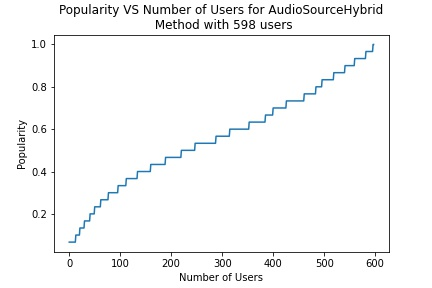
\includegraphics[scale=0.5]{CDF/AudioSourceHybrid_CDF.jpeg}}}%
    \qquad
    \subfloat[\centering Channel Merge Hybrid]{{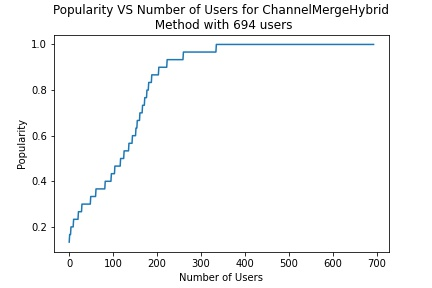
\includegraphics[scale=0.5]{CDF/ChannelMergeHybrid_CDF.jpeg}}}%
    \qquad
    \subfloat[\centering Amplitude Modulation Hybrid]{{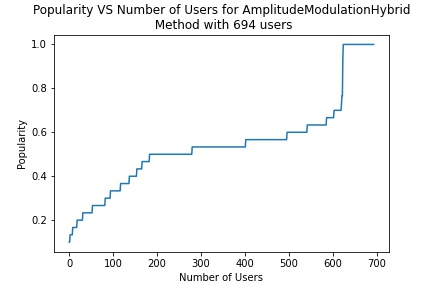
\includegraphics[scale=0.5]{CDF/AmplitudeModulationHybrid_CDF.jpeg}}}%
    \qquad
    \subfloat[\centering Frequency Modulation Hybrid]{{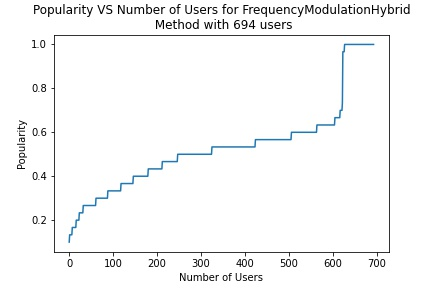
\includegraphics[scale=0.5]{CDF/FrequencyModulationHybrid_CDF.jpeg}}}%
    \caption[{The frequency of the highest occurring fingerprint value in 30 iterations for individual audio fingerprinting methods}]{The frequency of the highest occurring fingerprint value in 30 iterations for individual audio fingerprinting methods}
    \label{fig:CDFshowingAllFps}%
\end{figure}

\pagebreak{}

\end{appendices}

\phantomsection
\addcontentsline{toc}{chapter}{Vita}
\phantomsection

\chapter*{Vita}
The author, Saroj Duwal, was born in Bhaktapur, Nepal. He obtained his Bachelor's degree in Computer Science with a minor in Mathematics from the University of New Orleans in 2019. He joined the University of New Orleans Computer Science graduate program to pursue a Masters in Computer Science in Spring 2020. He has been working under Dr. Ben Samuels within the department of Computer Science at the University of New Orleans.

\end{document}
